\documentclass[10pt,a4paper]{report}
\usepackage[draft,inline,nomargin,index,marginclue]{fixme} 
\usepackage[utf8]{inputenc}
\usepackage[spanish]{babel}
\usepackage{amsmath}
\usepackage{graphicx}
\usepackage{braket}
\usepackage{amsfonts}
\usepackage{amssymb}
\author{Pablo Enrique Yanes Thomas}
\title{Candidatura}
\makeindex

\begin{document}

\tableofcontents
\chapter*{Objetivo General}
Si la frecuencia natural de un oscilador armónico mecánico con fricción,
acoplado a una cavidad de Fabry-Perot es una función periódica del
tiempo, el modelo de disipación usado debe tomar en cuenta esta dependencia; en
general esto no se hace. Durante el primer año de doctorado se encontró
que, si en este caso, se emplea un formalismo de disipación que toma en
cuenta la dependencia temporal de la frecuencia natural, se obtiene una
predicción cualitativa y cuantitativamente distinta para la temperatura
final del oscilador mecánico que si no se  toma en cuenta. Este
resultado justifica la sospecha de que en el caso de un sistema
optomecánico, en donde el oscilador mecánico también es un espejo
semitransparente, el cambio de la frecuencia natural de los modos de la
cavidad debe ser tomado en cuenta en el modelo de perdida de
fotones a través de los espejos. El objetivo de la tesis es investigar
esta posibilidad y sus posibles efectos en enfriamiento de sistemas
optomecánicos y manipulación de su estado cuántico.


\chapter{Introducción}

La optomecánica es el estudio de la interacción entre elementos ópticos y elementos mecánicos. En este capítulo se dará una breve introducción al tipo de sistemas y de efectos que se consideran parte de la optomecánica. 


\section{Posibles Sistemas Optomecánicos}

Existen muchas implementaciones posibles de acoplamientos entre elementos ópticos y elementos mecánicos \cite{KippenberCO}. En esta sección se detallan algunos de estos.

\subsection{Espejos Suspendidos}

Consisten de cavidades ópticas donde uno o más de los
espejos pueden cambiar de posición y así alterar la longitud de la
cavidad. La primera realización experimental de este tipo de sistemas
se debe a los primeros esfuerzos para detectar ondas gravitacionales
\cite{AbramoviciLIGO}. El sistema consiste en un interferómetro con
los espejos montados en masas suspendidas, a manera que una onda
gravitacional, al interactuar con las masas cambiaría la posición de
los espejos y así la longitud de camino óptico. El propósito de
suspender las masas no es crear un sistema optomecánico, sin embargo, fue necesario estudiar las fluctuaciones ocasionadas por la interacción entre la luz y las masas \cite{CavesIF}.
Experimentos en este tipo de sistemas han demostrado varios efectos,
entre ellos el enfriamiento mediante presión de radiación
\cite{CorbittOC}. También es posible utilizar este tipo de sistemas
para estudiar el entrelazamiento cuántico\cite{ChenED} al acoplar dos
cavidades al mismo espejo y así lograr entrelazamiento entre los modos
de ambos campos.

\subsection{Microresonadores}

Otro tipo posible de sistema optomecánico son los
microresonador o microcavidades. En este tipo de sistemas, es posible
confinar a la luz a viajar en modos \textit{whispering gallery}, los
cuales implican que la luz es guiada a lo largo del perímetro del
resonador, el cual puede tener forma esférica, circular, o
toroidal\cite{VahalaOM}. Si el resonador vibra, esto puede alterar el camino óptico de la luz y
se logra un acoplamiento entre el resonador macroscópico y la luz atrapada en el. Es posible fabricar resonadores de este tipo con un factor de calidad de $10^6$, este factor es igual a $2\pi$ veces el número de oscilaciones requeridas para que la energía almacenada en el resonador decaiga a $\frac{1}{e}$ de su valor inicial. Debido a su tamaño, es posible obtener acoplamiento fuerte entre sistemas cuánticos y el
resonador, el cual es un objeto macroscópico \cite{VerhagenMOC}.

\subsection{Objetos Suspendidos o Levitados}

En este tipo de sistemas, se considera una cavidad óptica rígida donde
se coloca un objeto mecánico dentro de la cavidad. Este esquema
permite el acoplamiento de objetos mecánicos de tamaños inferiores a
la longitud de onda de la luz \cite{KippenberCO}, como por ejemplo una
membrana dieléctrica de $SI_3N_4$ de $1mm \times 1mm \times 50nm$ de
dimensión\cite{SankeyMC}. En ese caso, se puede observar que
parámetros de la cavidad como la sintonización y la finesa dependen
del desplazamiento de la membrana. Otra posibilidad consiste en un
nano cable de carbón, de aproximadamente $10^9$ átomos, el cual se
coloca dentro de una micro cavidad de Fabri-Perot. Así mismo, se han
realizado experimentos donde se levita una gota de Helio líquido
dentro de la cavidad\cite{ChildressLD}. Las propiedades de la cavidad
cambian no solo dependiendo de la posición del objeto, sino también de
sus modos vibracionales\cite{FaveroCR}.

\subsection{Cristales Optomecánicos}

Este tipo de sistema es más reciente que los demás y se basa en redes
cristalinas donde se logra acoplar fotones y fonones. En uno de los primeros
experimentos se fabricó una nano viga
de silicio \cite{EichenfieldOC}. El sistema consiste en una nano viga
con agujeros espaciados de manera regular, lo cual forma una red. Se
introduce un defecto mediante una reducción cuadrática en la constante
de red, de manera simétrica respecto al centro de la viga. Esto genera un
potencial efectivo para los modos ópticos y uno análogo para los modos
mecánicos. Las vibraciones ocasionan un cierto desplazamiento en la
estructura lo cual afecta el potencial efectivo para los modos ópticos
y se obtiene el acoplamiento. Una implementación reciente de este tipo
de sistemas involucra usar redes cristalinas semi periódicas de
diamante para implementar el resonador\cite{BurekDO}.

\section{Efectos Optomecánicos}

En esta sección se da un pequeño resumen de los efectos 
 más conocidos y utilizados resultantes de la interacción optomecánica. Frecuentemente estos efectos
se deben a la interacción entre la presión de radiación que la luz
incidente aplica sobre los elemento mecánicos y la reacción retardada
de la cavidad a los cambios en su longitud o el equivalente en cavidades de otras geometrías.
Algunos de estos efectos son:


\begin{itemize}
\item \textbf{Efecto de Resorte Óptico (optical spring effect)} La
  presión de radiación depende de la posición del objeto, por lo que esta
  cambia cuando el objeto se mueve. En particular, en el caso de
  cavidades con espejos suspendidos, la presión de radiación afecta la
  constante del resorte ya que genera un desplazamiento en la
  resonancia de la frecuencia mecánica, el cual se puede utilizar para
  aumentar o disminuir la frecuencia natural del
  resorte.\cite{BraginskyPE}

\item \textbf{Bi-Estabilidad Óptica (optical bi-stability)} La presión
  de radiación puede desplazar al objeto mecánico y se espera que se
  llegue a una posición de equilibrio. Sin embargo, la dependencia del
  potencial efectivo sobre la posición es no lineal, lo cual lleva a
  que se generen dos posiciones de equilibrio. Para una presión lo
  suficientemente fuerte, este efecto se borra y se llega a una
  posición altamente estable\cite{DorselOB}.

\item \textbf{Enfriamiento Optomecánico} Este es el efecto en el que se basa este trabajo así que se describe en mayor detalle. 
\end{itemize}

\subsection{Enfriamiento Optomecánico}

En esta sección se da una breve explicación de la causa del enfriamiento optomecánico y la razón de que este sea un efecto puramente cuántico. La derivación se basa en la encontrada en \cite{WarwickQO} y requiere un teorema que se presenta sin demostración. Primero se define la  Densidad de Potencia Espectral como

\begin{equation}
S_{hh}(\omega) = \lim_{\tau \to\infty} \frac{1}{\tau}\langle h_\tau^*(\omega)h_\tau(\omega) \rangle ,
\end{equation} para h(t) una variable compleja cuyas propiedades estadísticas son independientes del tiempo. $h_\tau(\omega)$ es la transformada de Fourier tomada entre $\frac{-\tau}{2}< t < \frac{\tau}{2}$

\begin{center}
\textbf{Teorema de Wiener-Khinchin:} \textit{Sea h(t) una variable compleja cuyas propiedades estadísticas son estacionarias, entonces }

\begin{equation} \label{WienerKhichin}
S_{hh}(\omega) = \int_{-\infty}^\infty d\tau e^{i\omega \tau} \langle h^*(t+\tau)h(t) \rangle_{t=0} = \int_{-\infty}^\infty d\omega' \langle h^*(-\omega) h(\omega') \rangle
\end{equation}
.
\end{center}

El teorema es la primera igualdad y la segunda resulta de las propiedades de la transformada de Fourier. En el caso clásico la Densidad de Potencia Espectral es simétrica respecto a la frecuencia. Sin embargo, en el caso de operadores esto no es necesariamente cierto. Debido a que, en general, no se puede asegurar que para un operador Hermitiano $\hat{O}(t)$ se tenga $[\hat{O}(t),\hat{O}(t+\tau)] = 0$. Se sigue entonces que no se puede asegurar $S_{OO}(\omega) = S_{OO}(-\omega)$. El hecho de que un operador no necesariamente conmuta consigo mismo a distintos tiempos rompe la simetría. Se estudia ahora el caso específico de un oscilador armónico cuántico que está acoplado a un baño térmico mediante un término de tipo

\begin{equation}
V(t) = qF(t)
\end{equation} donde $F(t)$ es la fuerza ejercida por el baño, la cual conmuta con $q$. Se desea obtener la probabilidad de que el oscilador armónico pase de un estado inicial $\Ket{\Psi(t)}$  a un estado final ortogonal $\Ket{\Psi_f(t)}$. Se trabaja en el cuadro de interacción por simplicidad. En este caso la amplitud de transición $A_{if}(t)$ está dada por

\begin{equation}
A_{if}(t) =  \Braket{\Psi_f(t)|U_0 U_I|\Psi(0)}= e^{\frac{-i E_f t}{hbar}} \Braket{\Psi_f(t)|\Psi_I(t)} ,
\end{equation} donde

\begin{align}
U_0 =& e^{\frac{-i H_0 t}{\hbar}}\\
U_I =& e^{\frac{-i V t}{\hbar}}
\end{align} $H_0$ es el Hamiltoniano del oscilador armónico con frecuencia $\Omega$ y $V(t)$ es la interacción. Utilizando teoría de perturbación a primer orden, y asumiendo que la interacción es débil y por lo tanto los estados del baño y del oscilador armónico se mantienen separables, se llega a que la amplitud de transición para pasar de un estado $n$ a un estado $n+1$ en el oscilador, dado que el baño inicia en algún estado $j$ y que la interacción lo deje en un estado $k$ es

\begin{equation}
A_{if}(t) = \frac{x_{zp}\sqrt{n+1}}{i\hbar}\int_0^t d\tau_1 e^{i\Omega \tau_1} \Bra{k}F(\tau_1)\Ket{j},
\end{equation} donde $F_I(t)$ es la fuerza en el cuadro de interacción y $x_{zp}$ es la amplitud mínima del oscilador. La probabilidad de transición se obtiene al sumar sobre todos los posibles estados finales del baño y resulta

\begin{equation}
P_{n \to n+1} = \frac{x_{zp}^2 (n+1)}{\hbar^2} \int\int_0^t d\tau_1 d\tau_2 e^{i \Omega (\tau_2-\tau_1)}\langle F_I(\tau_1)F_I(\tau_2) \rangle ,
\end{equation} donde se ha utilizado que $F(t)$ es Hermitiana y que los modos del baño son completos. Se utilizan dos cambios de variable $\tau_1 = t' + \tau$ y $\tau_2 = t'$ para hacer más evidente la relación con \eqref{WienerKhichin}.

\begin{equation}
P_{n \to n+1} = \frac{x_{zp}^2 (n+1)}{\hbar^2} \int_0^t \int_{-t'}^{t-t'} dt' d\tau e^{i \Omega \tau}\langle F_I(t'+\tau)F_I(t') \rangle.
\end{equation} Si la integración se realiza con tiempos mucho más largos que los tiempos de auto-correlación del baño, los límites de la segunda integral se pueden aproximar por $\pm \infty$ y se llega a que

\begin{equation}
P_{n \to n+1} = \frac{x_{zp}^2 (n+1)}{\hbar^2} t S_{FF}(-\Omega).
\end{equation} Si se deriva respecto a $t$ se obtiene la taza de transición

\begin{equation}
\gamma_{n \to n+1} = \frac{x_{zp}^2 (n+1)}{\hbar^2}  S_{FF}(-\Omega),
\end{equation} y un cálculo análogo permite encontrar la taza de transición para $n \to n-1$ y esta resulta ser

\begin{equation}
\gamma_{n \to n-1} = \frac{x_{zp}^2 n}{\hbar^2} S_{FF}(\Omega).
\end{equation} Las transiciones que aumentan el número de excitaciones dependen de la parte negativa del espectro $S_{FF}$ mientras que las transiciones hacia abajo dependen de la parte positiva. De esta forma se espera que si se puede controlar el espectro de la fuerza ejercida por el baño se puede controlar que tipo de transición es dominante.
 


\section{Aplicaciones}

Existen muchas aplicaciones posibles para los efectos y sistemas utilizados en optomecánica. Este trabajo se concentra principalmente en enfriamiento optomecánico, sin embargo algunas otras posibles aplicaciones son:

\begin{itemize}

\item \textbf{Estabilización Láser} Al utilizar una cavidad de tipo cristal optomecánico doble (\textit{zipper cavity} en inglés) como base para un láser, se puede obtener un dispositivo tal que su frecuencia, en especial la sensibilidad de está a ruido térmico, se puede estabilizar optomecánicamente\cite{MayerZC}.

\item  \textbf{Memoria Optomecánica} Se puede crear un sistema de memoria utilizando una cavidad optomecánica compuesta por una guía de ondas y un resonador mecánico ligeramente torcido a manera de tener dos configuraciones posibles, arriba y abajo. Esto lleva a que se genere un potencial de doble pozo asimétrico para el resonador y, con la ayuda de un láser para excitar el sistema y de otro para enfriarlo, es posible realizar un proceso controlado donde se decide en que pozo queda el resonador. Estos dos estados corresponden a 0 y 1 y el sistema no requiere energía para mantenerse en la configuración final, generando un sistema de memoria estable \cite{BagheriMM}.

\item \textbf{Magnetometría} Al acoplar un material magnetostrictivo al resonador mecánico de una cavidad optomecánica se pueden excitar los eigenmodos del resonador mecánico al aplicar un campo magnético. De esta forma, la presencia del campo magnético se puede leer en el comportamiento del campo de luz dentro de la cavidad. Esto permite tener un sensor de campos magnéticos de alta precisión que funciona a temperatura ambiente \cite{ForstnerOM}.

\item \textbf{Redes Cuánticas} La optomecánica permite realizar el mapeo de los estados de un campo de luz a los modos vibracionales de un oscilador mecánico \cite{ZhangQST}. Este tipo de transferencia de información es clave en la formación de redes de información cuánticas.\cite{KimbleQI}

\item \textbf{Detección de Cáncer} Los Microtúbulos son una parte clave de la estructura de una célula y se ha estudiado si su interacción con campos electromagnéticos externos puede ser un tratamiento viable para el cáncer\cite{KirsonEMT}. El estudio de las propiedades vibracionales de estas estructuras es clave para esto y se ha propuesto un montaje experimental para realizar estas mediciones mediante un acoplamiento optomecánico\cite{SalariOC}.

\end{itemize} 

\section{Enfriamiento Optomecánico con Parámetros Dependientes del Tiempo}

Este trabajo se enfoca en el enfriamiento optomecánico con parámetros
dependientes del tiempo. Uno de los métodos empleados en la búsqueda
por mejorar el enfriamiento de un oscilador mecánico acoplado a una
cavidad es utilizar un oscilador mecánico cuya frecuencia natural sea
función del tiempo \cite{BarberisLC}. Esta dependencia modifica el
cuasi espectro de energía del sistema\cite{HanngiFM}. En el formalismo
empleado en \cite{BarberisLC} esto no se toma en cuenta, el efecto de la dependencia temporal sobre la disipación se modela mediante coeficientes con dependencia temporal que se introducen de manera ad-hoc.  Sin embargo, \cite{HanngiFM} muestra que este no es el enfoque óptimo, así que
realizó un trabajo que sí toma en cuenta los efectos de la dependencia
temporal de la frecuencia natural del oscilador durante la derivación
de la temperatura final que se espera del sistema \cite{YanesOC} y esta queda codificada en los operadores tanto del Hamiltoniano como de los términos de disipación e interacción. Los
resultados de este trabajo muestras diferencias cuantitativas y
cualitativas en el comportamiento de la temperatura del oscilador
mecánico, lo cual motiva la pregunta ¿Qué sucede al tomar en cuenta la
dependencia temporal de la frecuencia natural de la cavidad?

En esta propuesta se explican los pasos que se siguen para modelar
este tipo de sistemas en términos generales y luego se explica como se
obtiene la temperatura final del sistema. Finalmente se propone
aplicar este formalismo a un sistema donde se toma en cuenta la
dependencia temporal de la frecuencia de la cavidad. Se
discute la teoría de los sistemas cuánticos abiertos, del oscilador
mecánico dependiente del tiempo, y el enfriamiento optomecánico
dependiente del tiempo.




\chapter{Oscilador Armónico Dependiente del Tiempo}

Antes de proceder a enfriamiento optomecánico es importante saber como
modelar de manera cuántica un oscilador armónico con frecuencia
natural dependiente del tiempo. Para resolver este problema, se
utiliza la teoría de Floquet \cite{WardFT} y se busca una expresión
para el Hamiltoniano del sistema expresada en términos de operadores
de Floquet, los cuales se definirán más adelante.

\section{Teoría de Floquet}

Se desea resolver una ecuación diferencial que involucra coeficientes con dependencia temporal, tal como

\begin{equation}\label{FloquetEquation}
x' = A(t)x,
\end{equation} donde la función $A(t)$ es periódica con periodicidad $\tau$. En este caso el teorema de Floquet\cite{WardFT} dice que la solución no necesariamente es periódica pero debe tener la forma

\begin{equation}\label{FloquetForm}
x(t)=e^{\mu t}p(t).
\end{equation} Los valores $\mu$ se conocen como los exponentes característicos o de Floquet y la función $p(t)$ es periódica con período $\tau$, es decir el mismo periodo que el coeficiente en la ecuación diferencial. Los coeficientes $\mu$ son, en general, complejos. Claramente, el hecho de que la solución tenga la forma \eqref{FloquetForm} puede llevar a que la solución diverja con el tiempo, por lo que se desea entender el criterio de estabilidad para este tipo de soluciones. Antes de esto, es necesario establecer algunas definiciones y propiedades, las cuales se presentan sin demostración debido a que no son el enfoque principal de este trabajo. Si el lector se encuentra interesado, el tratamiento se encuentra con mayor detalle en las notas de las cuales surge la sección siguiente \cite{WardFT}.

\subsection{Propiedades Básicas}

Sea la ecuación \eqref{FloquetEquation} en $n$ dimensiones. Esto es,
se piensa en $x$ como un vector de $n$ dimensiones y en $A(t)$ como
una matriz de $n \times n$. En este caso, si la ecuación tiene $n$
soluciones $x_1, x_2, ... , x_n$, se define la \textbf{matriz
  fundamental} como la matriz formada utilizando las soluciones como
columnas, siempre y cuando estas sean linealmente independientes

\begin{equation}
X(t) = [[x_1][x_2]...[x_n]],
\end{equation}Si $X(t_0) = I$ la matriz se conoce como la \textbf{matriz fundamental principal}. Se tiene que

\begin{center}
\textbf{Lema:} \textit{Si $X(t)$ es una matriz fundamental, también lo es $X(t)C$ para cualquier matriz constante y no singular $C$.}
\end{center}Y que

\begin{center}
\textbf{Lema:} \textit{Sea $W(t)$, el Wronskiano de $X(t)$, también el determinante de $X(t)$,
  entonces:}

\begin{equation}
W(t) = W(t_0) e^{\int_{t_0}^{t}tr[A(s)]ds}.
\end{equation}
 
\end{center} Se tiene entonces un teorema

\begin{center}
\textbf{Teorema:} \textit{Sea A(t) una matriz con periodicidad $\tau$.
  Si $X(t)$ es una matriz fundamental entonces $X(t+\tau)$ también lo
  es y existe una única matriz constante no singular $B$ tal
  que:}\linebreak \linebreak i) $X(t+\tau) = X(t)B \qquad\forall t$,
\linebreak ii) $det(B) = e^{\int_0^t tr[A(s)]ds}.$
\end{center}
Si se toma $X(0)=I$ entonces $B=X(\tau)$. Con esto se pueden definir
los \textbf{multiplicadores característicos}, los cuales son los
valores propios de la matriz $B$, y se denominan con la letra $\rho$.
Estos cumplen que

\begin{equation}
\rho_1 = e^{\mu_1 \tau}, \quad \rho_2 = e^{\mu_2 \tau}, ... , \rho_n =
e^{\mu_n \tau},
\end{equation} donde los valores $\mu$ son los exponentes de Floquet definidos anteriormente. Se cumplen cuatro propiedades:

1) Los multiplicadores característicos de $B=X(\tau)$ cumplen que

\begin{equation}
det(B) = \rho_1 \rho_2 ... \rho_n = e^{\int_0^T tr[A(s)]ds}.
\end{equation}

2) Trivialmente, como la traza es la suma de los valores propios

\begin{equation}
Tr[B] = \rho_1 + \rho_2 + ... + \rho_n.
\end{equation}

3) Los multiplicadores característicos no son únicos, ya que

\begin{equation}
e^{\mu \tau} = e^{(\mu  +\frac{2\pi i}{\tau} )\tau}.
\end{equation}

4) Los multiplicadores característicos son una propiedad de la ecuación \eqref{FloquetEquation} y no dependen de la elección de matriz fundamental.

Con estas propiedades, se puede pasar a analizar la estabilidad de las soluciones para el caso específico de ecuaciones de segundo orden.

\subsection{Estabilidad para Ecuaciones de Segundo Orden}\label{EstabilidadSO}

Si se piensa en una ecuación diferencial de segundo orden del tipo

\begin{equation}
\ddot{x} + a(t)x= 0,
\end{equation} donde $a(t)$ tiene periodo $\tau$. Si se toma $x_1 = x$ y $x_2 = \dot{x}$, la ecuación puede re-escribirse como

\begin{equation}
[\begin{array}{c}
\dot{x_1} \\
\dot{x_2}
\end{array}] = [\begin{array}{cc}
0 & 1 \\
-a(t) & 0
\end{array}][\begin{array}{c} 
x_1 \\ 
x_2

\end{array}],
\end{equation} si se toma la condición inicial $[\begin{array}{c} 1 \\ 0 \end{array}]$, se obtiene una solución de la forma

\begin{equation}
[\begin{array}{c}
x_1^1(t) \\
\dot{x_1^1(t)}
\end{array}],
\end{equation} y para la condición inicial $[\begin{array}{c} 0 \\ 1 \end{array}]$, se obtiene una solución de la forma

\begin{equation}
[\begin{array}{c}
x_1^2(t) \\
\dot{x_1^2(t)}
\end{array}],
\end{equation} esto permite generar la matriz $B$

\begin{equation}
B= [\begin{array}{cc}

x_1^1(\tau) & x_1^2(\tau) \\
\dot{x_1^1(\tau)} & \dot{x_1^2(\tau)}

\end{array}],
\end{equation} lo cual permite calcular los multiplicadores característicos, ya que

\begin{equation}
\rho_1 \rho_2 = e^{\int_0^\tau Tr[A(s)]ds} = e^0 = 1,
\end{equation} y

\begin{equation}
 2\phi = \rho_1 + \rho_2 = Tr[B] =x_1^1(\tau)+ \dot{x_1^{(2)}(\tau)}.
\end{equation} Esto permite obtener la ecuación

\begin{equation}
\rho = \phi \pm \sqrt{\phi^2 -1},
\end{equation} o en términos de $\mu$

\begin{equation}
cosh(\mu_1 \tau) = \phi.
\end{equation} Esto lleva a analizar cinco situaciones distintas.

\textbf{Caso $ -1 < \phi < 1$}: En este caso, para algún valor $\sigma$ se tiene que $\phi = cos(\sigma \tau)$ por lo que:

\begin{align*}
\rho =& \phi \pm \sqrt{\phi^2 -1},\\
=& cos(\sigma \tau) \pm isen(\sigma \tau), \\
=& e^{\pm i\sigma \tau},
\end{align*} lo cual lleva a una solución general de tipo:

\begin{equation}
x(t) = c_1 Re(e^{i\sigma t} p(t)) + c_2 Im(e^{i\sigma t} p(t)),
\end{equation} la cual es estable y pseudo periódica.

\textbf{Caso $1 < \phi$:} en este caso $\rho > 1$ y como $\rho_1 = \frac{1}{\rho_2}$, tenemos que $\mu_1 = -\mu_2$. Por esto, la solución es de la forma:

\begin{equation}
x(t) = c_1 e^{\mu_1 t}p_1(t) + c_2 e^{\mu_2 t}p_2(t)
\end{equation} donde las funciones $p(t)$ son periódicas con periodo $\tau$. 
La solución es inestable.

\textbf{Caso $\phi < -1$:} en este caso se tiene una solución del
tipo:

\begin{equation}
x(t) =c_1 e^{\gamma_1 t}q_1(t) + c_2 e^{-\gamma_2 t}q_2(t),
\end{equation} donde las funciones $q(t)$ tienen periodo $2\tau$ y los coeficientes $\gamma = \mu + \frac{i\pi}{\tau}$. La solución de nuevo es inestable.

\textbf{Caso $\phi = -1$:} para este caso también se tiene una
solución inestable, de la forma:

\begin{equation}
x(t) = (c_1 + tc_2)q_1(t) + c_2q_2(t)
\end{equation} de nuevo la funciones $q(t)$ tienen periodo $2\tau$.

\textbf{Caso $\phi = 1$:}

para este caso también se tiene una solución inestable, de la forma:

\begin{equation}
x(t) = (c_1 + tc_2)p_1(t) + c_2p_2(t)
\end{equation} de nuevo la funciones $p(t)$ tienen periodo $\tau$.

Es muy importante notar que en estos dos últimos casos, esta forma de la solución solo es correcta si la matriz $B$ tiene un solo eigenvector linealmente independiente. Si este no es el caso, la solución tiene la forma usual con las funciones $p(t)$ o $q(t)$, estos dos casos marcan el límite entre la estabilidad y la inestabilidad en este problema. Finalmente, se verá como estos criterios aplican a una ecuación que será relevante más adelante, la ecuación de Hill.

\subsection{Estabilidad de las Soluciones de Floquet para la Ecuación de Hill}

La ecuación de Hill es una ecuación diferencial de segundo orden con coeficientes dependientes del tiempo de forma periódica\cite{WardFT}

\begin{equation}
\ddot{x}(t) + (\delta + \epsilon b(t))x = 0,
\end{equation} nuevamente, la función $b(t)$ tiene periodo $\tau$ y se considera que $\delta$ y $\epsilon$ son constantes reales. Para el caso $\epsilon = 0$ claramente la ecuación se reduce al oscilador armónico usual y las soluciones son estables. Sin embargo, para ciertos valores de $\delta$ puede encontrarse la región donde la solución aún es periódica, esto se puede resolver para los casos $\phi = \pm 1$, donde $\phi$ es la función definida en la sección \eqref{EstabilidadSO}, de forma que se tiene soluciones estables y periódicas para los casos

\begin{equation}
\delta = (2m\frac{\pi}{\tau})^2, 
\end{equation} que corresponde a $\phi=1$ y

\begin{equation}
\delta = ((2m+1)\frac{\pi}{\tau})^2,
\end{equation}
que corresponde a $\phi=-1$. Estos valores representan la frontera de
la región de soluciones estables, las cuales corresponden a periodo de
$\tau$ y $2\tau$ respectivamente. A continuación se buscaran soluciones
en esta región para el caso donde $\epsilon \ll 1$.

\subsection{Solución para Oscilaciones Pequeñas}

Se estudia un ejemplo cuyos resultados se utilizan más adelante. Se toma como función periódica una función constante más una pequeña perturbación periódica. Se emplea el ejemplo de que esta función sea la frecuencia natural de un oscilador armónico.

\begin{equation}\label{SmallOscillationsTDHO}
\nu(t) = \nu_0 + \epsilon cos(2\omega t),
\end{equation} donde $\epsilon \ll \nu_0$ y $\nu_0$ es la frecuencia natural promedio. Esto lleva a una ecuación de oscilador armónico

\begin{equation}
\ddot{x} + (\nu_0^2 + 2\epsilon \nu_0 cos(2\omega t))x = 0,
\end{equation} la cual es un caso particular de la ecuación de Mathieu \cite{PiatekME}. A fin de tener la ecuación en la forma estándar hacemos $t'= \omega t$ y $\epsilon' = \frac{2\epsilon \nu_0}{\omega^2}$ y


\begin{equation}
\frac{\nu_0^2}{\omega^2} = n^2\label{scattering}
\end{equation}

con $n \in \mathbb{Z}^+$ ya que como se vio esto es necesario para tener soluciones estables\cite{WardFT}. Bajo estas restricciones, tenemos que las soluciones para \eqref{SmallOscillationsTDHO} son, a primer orden en $\epsilon$ y para $n=1$

\begin{equation}\label{SmallOscillationsSolution}
f(t)=  e^{i\omega t} + \frac{\epsilon}{16} e^{3i\omega t},
\end{equation} y su complejo conjugado es $f(-t)$.


\section{Estados de Floquet en Mecánica Cuántica}

Utilizaremos los resultados obtenidos en la
  sección anterior para estudiar Hamiltonianos con un parámetro con
  una dependencia periódica en el tiempo

\begin{equation} \label{TimeH}
H(t)=H(t+\tau).
\end{equation} El hecho de que el Hamiltoniano sea simétrico respecto a (ciertas) traslaciones en el tiempo, permite el uso del formalismo de Floquet \cite{HanngiDQS}. Se asume que la dependencia temporal puede ser vista como una perturbación sobre un Hamiltoniano original

\begin{equation}
H(x,t)=H_0(x)+V(x,t) \qquad V(x,t)=V(x,t+\tau).
\end{equation}
Se utiliza que el Hamiltoniano no perturbado posee un conjunto
completo de eigenfuciones $\{\phi_n\}$ con valores propios
correspondientes $E_n$.   La
ecuación de Schr\"{o}dinger tiene la forma

\begin{equation}\label{SchrodingerEQ}
-i\hbar\dot{\Psi}(x,t) = H(x,t)\Psi(x,t).
\end{equation} El problema cumple con las condiciones necesarias para utilizar una solución del tipo visto en la sección anterior

\begin{equation}
\Psi_n(x,t) = e^{(\frac{-i}{\hbar}\mu_nt)}\Phi_n(x,t).
\end{equation} Como se mencionó en la sección anterior, $\mu$ en general es un número complejo, lo cual puede llevar a soluciones inestables. En este caso $\Phi_n(x,t)$ es la función que contiene la periodicidad en el tiempo. Sustituir la solución en la ecuación \eqref{SchrodingerEQ} genera una ecuación para las funciones periódicas

\begin{equation}
H(x,t)\Phi_n(x,t)=E_n\Phi_n(x,t).
\end{equation} Antes de buscar formas explícitas para estos estados, es necesario resolver el problema clásico correspondiente a este sistema. La razón para esto se verá más adelante, y se debe sencillamente a que estas soluciones clásicas juegan un papel clave en las expresiones explícitas para los estados y operadores involucrados en la solución del problema cuántico.

\section{Oscilador Armónico Dependiente del Tiempo: Solución Mediante Formalismo de Floquet}

En el caso clásico \cite{HanngiFM} se tiene, para un oscilador armónico unidimensional con frecuencia dependiente del tiempo y el cual experimenta una fuerza disipadora dependiente de la velocidad, que la posición cumple

\begin{equation}
\ddot{x}+\gamma\dot{x}+\frac{k(t)}{m}x=0
\end{equation}

Se asume que la función $k(t)$ es periódica con periodo $T$. Si se utiliza la sustitución $x=ye^{-\frac{\gamma t}{2}}$, se llega a la ecuación

\begin{equation}
\ddot{y} +(\frac{k(t)}{m}-\frac{\gamma^2}{4})y=0
\end{equation}

El teorema de Floquet para ecuaciones de segundo orden con
coeficientes dependientes del tiempo \cite{HanngiFM} asegura
que esta ecuación tiene dos soluciones

\begin{equation}
f_1(t) = e^{i\mu t}\Phi(t), \quad f_2(t)=f_1(-t),
\end{equation}
Recordando que la función $\Phi$ debe tener la misma periodicidad que
$k(t)$. En el caso de un Hamiltoniano con dependencia temporal como la de \eqref{TimeH}, existe un conjunto completo de soluciones
\cite{BarnettSD}

\begin{equation}
\Ket{\Psi_\alpha (t)} = e^{-i\mu_\alpha t}\Ket{\Phi_\alpha t}, \qquad \Ket{\Phi_\alpha (t)}=\Ket{\Phi_\alpha (t+\tau)},
\end{equation}

Estas soluciones tienen la forma explícita\cite{BrownPT}

\begin{equation}
\Psi_\alpha (x,t) = (\frac{\sqrt{m/\pi\hbar}}{2^\alpha n! f_1^0(t)})^{\frac{1}{2}}(\frac{f_1^0(t)}{f_2^0(t)})^\frac{\alpha}{2}H_\alpha(x\sqrt{\frac{m}{\hbar f_1^0(t) f_2^0(t)}})e^{(ix^2\frac{f_1^0(t)}{2f_2^0(t)})}
\end{equation} donde el superíndice cero indica que se toma el límite donde $\gamma$ tiende a cero. Sin embargo, estas soluciones se comportan de manera análoga a los estados de la base de Fock bajo la acción de los operadores de Floquet, los cuales pueden expresarse en términos de los operadores de momento y posición usuales en mecánica cuántica

\begin{equation}\label{FloquetOperators}
\Gamma(t) = \frac{1}{2i}(\hat{x}\dot{f}_1^0(t)\sqrt{\frac{2}{\hbar m}}-\hat{p}f_1^0(t)\sqrt{\frac{\hbar}{2m}}).
\end{equation} Así como su complejo conjugado. Su acción sobre la base de Floquet queda definida por

\begin{align*}
\Gamma(t) \Ket{\Psi_\alpha (x,t)} =& \sqrt{\alpha}\Ket{\Psi_{\alpha-1} (x,t)}, \\
\Gamma^\dagger(t) \Ket{\Psi_\alpha (x,t)} =& \sqrt{\alpha+1}\Ket{\Psi_{\alpha+1} (x,t)}.
\end{align*}Es importante notar que estos operadores dependen explícitamente del tiempo. Es conveniente entender el origen de estos operadores. 

Sea un Hamiltoniano usual de oscilador armónico, con la excepción de que la frecuencia natural del oscilador es una función periódica del tiempo

\begin{equation}\label{TDHO}
H = \frac{1}{2m}p^2 + \frac{1}{2}k(t)q^2.
\end{equation} Este lleva a la ecuación de movimiento usual

\begin{equation}
m\ddot{q}(t) + k(t)q(t) = 0,
\end{equation} para el operador $q(t)$. Lo que se busca es una transformación unitaria que lleve este problema al problema usual del oscilador armónico en mecánica cuántica. Se trabaja en el cuadro de Heisenberg \cite{SakuraiQM}, tal que

\begin{align}
\tilde{q}(t) =& U^{-1}(t)q(t)U(t),\\
\tilde{p}(t) =& U^{-1}(t)p(t)U(t).
\end{align} Y donde entonces el nuevo Hamiltoniano queda dado por

\begin{equation}
\tilde{H} = H + U^{-1}i\dot{U}.
\end{equation} Para la transformación se elige

\begin{equation}
U = e^{-i\chi(t)q^2(t)},
\end{equation} donde

\begin{equation}
\chi(t) = \frac{m}{4}(\frac{\dot{f}}{f}+\frac{\dot{f^*}}{f^*})
\end{equation} Las funciones $f$ son las soluciones al problema clásico correspondiente al Hamiltoniano \eqref{TDHO} el cual tiene dos soluciones linealmente independientes, pero una es la compleja conjugada de la otra. Estas soluciones corresponden a las funciones $f_1^0$  y $f_2^0$ vistas en la sección anterior. Bajo esta transformación

\begin{align}
\tilde{q}(t)=&q(t),\\
\tilde{p}(t)=&p(t)-2\chi(t)q(t).
\end{align} Se puede escribir el Hamiltoniano en las nuevas coordenadas tomando en cuenta que $\ddot{f}= -k(t)f$

\begin{equation}
 H = \frac{1}{2m}\tilde{p}^2 + \frac{\chi(t)}{m}(\{\tilde{q},\tilde{p}\}) + \frac{mW^2}{|f|^2}k(t)\tilde{q}^2,
\end{equation} donde W es el Wronskiano

\begin{equation}
W=\frac{1}{2i}(\dot{f}(t)f^*(t)-f(t)\dot{f}^*(t)).
\end{equation} Para eliminar el término cruzado se utiliza una segunda transformación unitaria

\begin{equation}
U_2(t)=e^{\frac{i}{4}(\{\tilde{q},\tilde{p}\})ln|f|^2}.
\end{equation} Al aplicar esta transformación a las variables $\tilde{q}$ y $\tilde{p}$ se obtienen las variables finales $Q$ y $P$ las cuales son

\begin{align}
Q=&U_2^{-1}\tilde{q}U_2 = \frac{\tilde{q}}{|f|} =\frac{1}{|f|}q,\\
P=&U_2^{-1}\tilde{p}U_2 = |f|\tilde{p} =|f|(p-2\chi q), 
\end{align} El Hamiltoniano se reescribe en estas nuevas variables y se obtiene

\begin{equation}\label{QTDHO}
\tilde{H} = \frac{1}{|f(t)|^2}(\frac{1}{2m}P^2(t)+\frac{1}{2}mW^2Q^2(t)).
\end{equation}Este Hamiltoniano es, salvo por un coeficiente general dependiente del tiempo, el Hamiltoniano usual de oscilador armónico y se puede resolver por medio de operadores de escalera

\begin{equation}
\Gamma = \sqrt{\frac{mW}{2}}Q + i \sqrt{\frac{1}{2mW}}P.
\end{equation} La expresión \eqref{FloquetOperators} se obtiene expresando los operadores en las coordenadas usuales, no en las transformadas. Es de mas utilidad expresar este Hamiltoniano en términos de estos operadores $\Gamma(t)$. Se obtiene

\begin{equation}
\tilde{H} = \frac{W}{|f(t)|^2}(\Gamma^\dagger(t)\Gamma(t) + \frac{1}{2}).
\end{equation}

Con esto establecido se puede proceder a establecer un Hamiltoniano para enfriamiento optomecánico con parámetros dependientes del tiempo.



\chapter{Enfriamiento Optomecánico Dependiente del Tiempo: Caso de Oscilador Armónico Dependiente del Tiempo}

En este capítulo se da un breve resumen del trabajo realizado en \cite{TesisMaestria} y en \cite{YanesOC}. Se muestra que  cuando se toma en cuenta una dependencia temporal en la frecuencia  de un oscilador armónico mecánico acoplado a una cavidad de Fabry-Perot se llega a cambios cuantitativos y cualitativos en el enfriamiento del mismo siempre y cuando se utilice un modelo de disipación que incorpore esta dependencia. Esto motiva el trabajo que inicia en el capítulo siguiente.


\section{Hamiltoniano para Enfriamiento Optomecánico con Parámetros Dependientes del Tiempo}

Se estudia un sistema compuesto por una cavidad óptica de Fabry-Perot donde uno de los dos espejos se encuentra acoplado a un oscilador armónico mecánico, lo cual le permite moverse. La frecuencia natural del oscilador mecánico es una función periódica del tiempo. Se asume que el oscilador interactúa únicamente con un modo de la cavidad  con frecuencia $\omega_{cav}$, dicho modo se encuentra forzado por un láser.Se asume que el marco de referencia rota con la frecuencia del láser de forzamiento. Se modela el sistema mediante el siguiente Hamiltoniano\cite{BarberisLC}

\begin{equation}
H(t) = H_{cav} + H_{mec}(t) + H_{rad} + H_{laser}.
\end{equation} En donde

\begin{align}
H_{cav} =& -\hbar \delta a^\dagger a,\\
H_{mec}(t) =& \frac{p^2}{2m} + \frac{1}{2}m \nu^2 (t) x^2,\\
H_{rad} =& -\hbar g a^\dagger a x,\\
H_{laser} =& \hbar\frac{\Omega}{2}(a^\dagger + a),
\end{align} en este caso, $\delta = \omega_{laser} - \omega_{cav}$ representa la diferencia de frecuencias entre el láser de forzamiento y la cavidad y $\hbar g$ representa la fuerza de radiación que un fotón ejerce sobre el oscilador mecánico sin modulación. El término $H_{rad}$ modela una interacción simple entre los fotones y el espejo. Dado que en este caso la longitud de la cavidad no es fija, la frecuencia de la cavidad debe tener una dependencia en la coordenada $x$. Una derivación completa de este término puede encontrarse en la referencia \cite{KippenberCO}. Por \eqref{QTDHO}, se modela al oscilador mecánico utilizando operadores de Floquet

\begin{equation}
H_{mec}(t) = \hbar\frac{W}{|f(t)|^2}(\Gamma^\dagger \Gamma + \frac{1}{2}).
\end{equation} Recordando la definición de los operadores de Floquet \eqref{FloquetOperators}, se puede invertir la relación en términos de los operadores $x$ y $p$ y sustituir el resultado en el Hamiltoniano de interacción, lo cual produce un nuevo Hamiltoniano de interacción\cite{TesisMaestria}

\begin{equation}
H(t)_{rad} = 2ig\sqrt{\frac{\hbar^3}{2m}}  a^\dagger a[\gamma_+(t)\Gamma (t) +\gamma_-(t)\Gamma^\dagger (t)]
\end{equation} donde

\begin{align}
\gamma(t)_+ =& \frac{i}{4}\sqrt{\frac{2}{m\hbar^3}} \frac{f(t)^*}{(\dot{f}(t)f(t)^*-\dot{f}(t)^*f(t))},\\
\gamma(t)_- =& \frac{i}{4}\sqrt{\frac{2}{m\hbar^3}} \frac{f(t)}{(\dot{f}(t)f(t)^*-\dot{f}(t)^*f(t))},
\end{align} con esto, el Hamiltoniano final es el siguiente

\begin{equation}\label{LaserCoolingHamiltonian}
H(t) = -\hbar \delta a^\dagger a + \frac{W}{|f(t)|^2}(\Gamma^\dagger \Gamma + \frac{1}{2}) +  g'a^\dagger a[\gamma_+(t)\Gamma (t) +\gamma_-(t)\Gamma^\dagger (t)] + \hbar\frac{\Omega}{2}(a^\dagger + a),
\end{equation} donde 

\begin{equation}
g'=g\sqrt{\frac{\hbar^3}{2m}}.
\end{equation}

Sin embargo el Hamiltoniano no es suficiente, se utiliza el formalismo de ecuaciones maestras a fin de modelar la disipación. Se utiliza un modelo de disipación que incorpora los operadores de Floquet y por ende la dependencia temporal del oscilador durante todo el proceso de derivación. 

\section{Disipación en Sistemas Optomecánicos}

Las ecuaciones maestras modelan la evolución temporal de un sistema donde puede haber intercambios de energía con el medio ambiente, al cual se le conoce usualmente como reservorio térmico. En este caso se desea modelar un oscilador armónico mecánico que puede intercambiar energía con el campo electromagnético dentro de una cavidad. Se toma en cuenta que la cavidad pierde fotones al exterior. Para una derivación de este tipo de ecuaciones, el lector puede consultar\cite{ZollerQN}. La ecuación es muy similar a la ecuación de Liouville, ya que se estudia la evolución temporal de la matriz densidad del sistema. Normalmente este tipo de ecuaciones requieren de dos aproximaciones. La aproximación de Born donde se asume que la interacción es lo suficientemente débil como para descartar términos de mayor a segundo orden en la misma y la aproximación de Markov, donde se asume que el reservorio térmico no cambia su estado debido a su interacción con el resto del sistema y de esta forma no actúa como un tipo de memoria para este\cite{CarmichaelFL}. Estas ecuaciones tienen la forma general

\begin{equation}\label{MasterEq}
\dot{\rho} = \frac{1}{i\hbar}[H,\rho] + L\rho,
\end{equation} donde $\rho$ es la matriz densidad del sistema, $H$ es el Hamiltoniano que modela el sistema sin tomar en cuenta intercambios de energía con un reservorio y $L$ es el superoperador de Lindblad, el cual codifica el efecto de la parte abierta del sistema, es decir la parte del sistema que puede interaccionar con el medio ambiente y causar intercambios de energía.

Se busca modelar las interacciones entre un oscilador armónico mecánico y un campo electromagnético de un modo el cual actúa como baño térmico. El campo electromagnético puede perder fotones al medio ambiente. Esto corresponde a dos términos de Lindblad. Debido a que los Hamiltonianos para el campo dentro de la cavidad y para el oscilador armónico mecánico tienen la misma forma algebraica y sus operadores siguen las mismas reglas de conmutación los términos de Lindblad tienen formas idénticas. Estos son \cite{EnglertDB}

\begin{align}
L_a \rho =& - \frac{\kappa}{2}(n_p + 1)[a^\dagger a\rho + \rho a^\dagger a -2a\rho a^\dagger]  \\
 &- \frac{\kappa}{2}(n_p)[ aa^\dagger\rho + \rho  aa^\dagger -2a^\dagger\rho a].\nonumber
\end{align}
 Y 
\begin{align}
L_\Gamma \rho =& - \frac{\gamma}{2}(n_m + 1)[\Gamma^\dagger \Gamma\rho + \rho \Gamma^\dagger \Gamma -2\Gamma\rho \Gamma^\dagger]  \\
 &- \frac{\gamma}{2}(n_m)[ \Gamma\Gamma^\dagger\rho + \rho  \Gamma\Gamma^\dagger -2\Gamma^\dagger\rho \Gamma].\nonumber
\end{align} tal que


\begin{equation} \label{MasterEquation}
\dot{\rho} = \frac{1}{i\hbar}[H,\rho] + L_\Gamma \rho + L_a \rho
\end{equation} 

Esta ecuación es uno de los resultados presentados en \cite{YanesOC}. En este caso $\kappa$ es el coeficiente de disipación dentro de la cavidad y $\gamma$ es el coeficiente de disipación para el oscilador armónico mecánico. En estudios anteriores de este tipo de sistemas la dependencia temporal de la frecuencia se incorporaba mediante este coeficiente de manera ad-hoc \cite{BarberisLC}, sin embargo el emplear operadores de Floquet toma en cuenta los efectos de la aproximación de Markov sobre el quasi espectro de energía del sistema\cite{HanngiFM}. $n_p$ y $n_m$ son los números de excitaciones térmicas fotónicas y mecánicas y $a$ y $a^\dagger$ son los operadores de escalera usuales para el oscilador armónico, mientras que $\Gamma$ y $\Gamma^\dagger$ son los operadores de Floquet.



\section{Transformación Mediante Operador de Desplazamiento}\label{Desplazamiento}

Para poder proceder es necesario eliminar los términos de tercer orden en operadores, ya que estos son no-lineales y causan dificultades. Esto se logra mediante una transformación unitaria. Se utiliza la transformación

\begin{equation}
U_{a,\Gamma} = e^{(\alpha(t) a^\dagger - \alpha(t)^*a)}e^{(\beta(t) \Gamma^\dagger - \beta(t)^*\Gamma)},
\end{equation} Tanto $\alpha$ como $\beta$ dependen del tiempo, está dependencia no se escribirá de forma explícita a futuro por brevedad. Bajo la transformación, el operador densidad es

\begin{equation}
\rho' = U_{a,\Gamma}^\dagger \rho U_{a,\Gamma}.
\end{equation} Se puede despejar en términos de $\rho$, aprovechando que la transformación es unitaria

\begin{equation}
\rho = U_{a,\Gamma} \rho' U_{a,\Gamma}^\dagger,
\end{equation} y derivando respecto al tiempo

\begin{equation}
\dot{\rho} = L\rho = \frac{d}{dt}(U_{a,\Gamma} \rho' U_{a,\Gamma}^\dagger).
\end{equation} En este caso, $L$ representa el operador de Liouville. Esto permite obtener una ecuación maestra para $\rho$. 

\begin{align}
 U_{a,\Gamma} \dot{(\rho')} U_{a,\Gamma}^\dagger =& L[U_{a,\Gamma} \rho' U_{a,\Gamma}^\dagger] - \dot{U}_{a,\Gamma}\rho'U_{a,\Gamma}^\dagger -U_{a,\Gamma} \rho' \dot{U}_{a,\Gamma}^\dagger\\
\dot{\rho} =& U_{a,\Gamma}^\dagger L[U_{a,\Gamma} \rho' U_{a,\Gamma}^\dagger]U_{a,\Gamma}-U_{a,\Gamma}^\dagger\dot{U}_{a,\Gamma}\rho'-\rho'\dot{U}_{a,\Gamma}^\dagger U_{a,\Gamma}.
\end{align}

Esta transformación se emplea de nuevo y con más detalle en el capítulo siguiente. En el caso donde $\alpha$ y $\beta$ cumplen con las ecuaciones

\begin{align}
\dot{\alpha} =& \alpha(-\frac{A}{2}+i(\delta+g'(\gamma_-(t) \beta^* + \gamma_+(t) \beta))-i\frac{\Omega}{2},\\
\dot{\beta} =& \beta(-\frac{\gamma}{2}-i\frac{W}{|f(t)|^2})+ig'|\alpha|^2\gamma_+(t),
\end{align} el Hamiltoniano resulta


\begin{align*}
H'=& -\hbar \delta' a^\dagger a + \frac{W}{|f(t)|^2}\Gamma \Gamma^\dagger -\hbar g'[(a^{\dagger}a +\alpha a^{\dagger}+\alpha^* a)(\gamma_-(t)\Gamma^{\dagger}+\gamma_+(t)\Gamma)]\\
&+ i\hbar(\beta^*\dot{\Gamma} - \beta \dot{\Gamma}^\dagger),
\end{align*}  donde se ha hecho el cambio $\delta' = \delta + g'(\beta + \beta^*)$. Con esto se obtiene la ecuación maestra para el enfriamiento optomecánico con un oscilador con frecuencia dependiente del tiempo, en el marco de referencia desplazado


\begin{equation}\label{DLCMasterEquation}
\dot{\rho} = \frac{1}{i\hbar}[H',\rho] + L_a\rho + L_\Gamma\rho + |\beta|^2(Re[C])\rho,
\end{equation} donde 

\begin{equation}
C = [\dot{\Gamma}^\dagger, \Gamma]
\end{equation} 


\subsection{Solución Explícita para Pequeñas Oscilaciones }

Con una solución para el caso de una frecuencia como en\eqref{SmallOscillationsTDHO}  en mano, podemos calcular soluciones explícitas para todos los términos que se han obtenido. Estos resultan ser\cite{TesisMaestria}

\begin{equation}
C(t) = i [1 -\frac{\epsilon}{16}e^{-2i\omega t}-\frac{6\epsilon}{16}e^{2i\omega t}].
\end{equation} Los coeficientes $\gamma_{\pm}$ son

\begin{equation}
\gamma_\pm= \frac{1}{\omega}e^{\mp i\omega t},
\end{equation} se hace lo mismo para el factor global en el Hamiltoniano de oscilador armónico en operadores de Floquet

\begin{equation}
\frac{W}{|f|^2} = \omega.
\end{equation} 

Y se puede obtener expresiones explícitas para los coeficientes $\alpha(t)$ y $\beta(t)$ en la transformación al marco desplazado

\begin{align}
\dot{\alpha} =& \alpha(-\frac{A}{2}+i(\delta+g'(e^{i\omega t} \beta^* + e^{-i\omega t} \beta)))-i\frac{\Omega}{2},\\
\dot{\beta} =& \beta(-\frac{\gamma}{2}-i 2\omega)+ig'|\alpha|^2e^{i\omega t},
\end{align} asumiendo que $\alpha$ y $\beta$ lleguen a su estado estacionario de manera suficientemente rápida se puede tomar $\dot{\alpha}(t)=\dot{\beta}(t)=0$ y se trabaja
en el régimen de acoplamiento débil por lo que coeficientes de orden
mayor a cero en $g'$ se desprecian. Esto lleva a

\begin{align}
0 =& \alpha(-\frac{A}{2}+i\delta)-i\frac{\Omega}{2},\\
0 =& \beta(-\frac{\gamma}{2}-i 2\omega),
\end{align} cuya solución es trivial 

\begin{align}
\alpha_0 =& \frac{\Omega}{2\delta-iA},\\
\beta_0 =& 0.
\end{align} El subíndice 0 muestra que las soluciones son válidas a orden cero en el acoplamiento. Bajo estás condiciones  el Hamiltoniano resulta

\begin{align}
H(t) =& -\hbar \delta a^{\dagger}a +\hbar\omega\Gamma^{\dagger}\Gamma \\
&-\hbar g'(a^{\dagger}a +\alpha_0 a^{\dagger}+\alpha^*_0 a)(\gamma_-(t)\Gamma^{\dagger}+\gamma_+(t)\Gamma)\nonumber.
\end{align}
Se trabaja en el régimen donde $|\alpha_0| \gg 1$
\cite{BarberisLC}, por lo que el término $a^\dagger a$ se puede
despreciar y se llega a un Hamiltoniano simplificado

\begin{align} \label{LCHamiltonian}
H(t) =& -\hbar \delta a^{\dagger}a +\hbar\omega\Gamma^{\dagger}\Gamma \\
&+\frac{\hbar g'}{\omega}(\alpha_0 a^{\dagger}+\alpha^*_0 a)(e^{i\omega t} \nonumber\Gamma^{\dagger}+e^{-i\omega t}\Gamma)
\end{align}

Este Hamiltoniano genera la ecuación maestra \eqref{MasterEquation}

\begin{equation}\label{LCMasterEq}
\dot{\rho} = \frac{1}{i\hbar}[H,\rho] +L_a\rho + L_\Gamma \rho,
\end{equation} 


\subsection{Base de Decaimiento}

En el caso de ecuaciones maestras correspondientes a un Hamiltoniano
de tipo oscilador armónico,una de las posibles soluciones es mediante la base de decaimiento\cite{EnglertDB}. Esta solución es particularmente conveniente puesto que más adelante será necesario tomar trazas sobre todos los grados de libertad de la cavidad, lo cual resulta relativamente sencillo en esta base.

\begin{equation}\label{Englert1993}
\rho_\lambda (a,a^\dagger) = :f(aa^\dagger):a^l.
\end{equation} Los $::$ denotan ordenamiento normal, lo cual puede requerir el desarrollo en serie de la función $f$. Se puede expresar $a^l$ en la base de número como

\begin{equation}
\sum_{n=0}^\infty C_n^l\Ket{n}\Bra{n+l},
\end{equation}

Es importante notar que $L$ no es necesariamente auto-adjunto, por lo que no se puede garantizar que sus funciones propias formen una base completa del espacio ni que sus valores propios sean reales. En el caso de este tipo de operadores existen dos tipos de vectores propios\cite{BarnettSD}, izquierdos y derechos

\begin{align*}
L\rho =& \lambda \rho, \\
\check{\rho} L =& \lambda \check{\rho}.
\end{align*} Los estados que se obtienen al aplicar el súper-operador por la derecha se conocen también como estados duales, se denotan por $\check{\rho}$. También es importante notar que los vectores que se obtienen al aplicar por la izquierda y por la derecha no son simplemente complejos conjugados uno del otro, se conocen como duales y son ortogonales los unos a otros bajo un producto definido mediante la traza\cite{EnglertDB}, sin embargo sus valores propios son iguales. Los vectores obtenidos no forman necesariamente una base del espacio de operadores. 

\begin{equation}
Tr[\check{\rho}_\lambda \rho_{\lambda'}] = \delta_{\lambda'\lambda}.
\end{equation} Esto se puede emplear para obtener las constantes de la expansión

\begin{equation}
\rho(0) = \sum_{\lambda} \check{c}_{\lambda} \rho_{\lambda},
\end{equation} donde

\begin{equation}
\check{c}_\lambda = Tr[\check{\rho}_\lambda \rho(0)].
\end{equation}

A partir de este se llega a la solución para los estados izquierdos $\rho_n^l$, los cuales corren sobre dos índices discretos y corresponden a los valores propios
\cite{EnglertDB}

\begin{equation}
\lambda_n^l = -\kappa[n + \frac{|l|}{2}],
\end{equation} los cuales cumplen con las condiciones

\begin{equation}
n=0,1,2...,\qquad l = 0,\pm 1, \pm 2,... 
\end{equation} y estos estados son

\begin{align}\label{DefDB}
&a^{\dagger l}\frac{(-1)^n}{(\nu+1)^{l+1}}:L_n^l[\frac{a^\dagger a}{\nu+1}]e^{-[\frac{a^\dagger a}{\nu+1}]}:\quad l \geq 0, \\
&\frac{(-1)^n}{(\nu+1)^{|l|+1}}:L_n^{|l|}[\frac{a^\dagger a}{\nu+1}]e^{-[\frac{a^\dagger a}{\nu+1}]}:a^{|l|}\quad l \leq 0,
\end{align} donde $L_n^l$ son los polinomios asociados de Laguerre. Es importante notar que esto se obtiene en el cuadro de interacción,
por lo que los eigenvalores fuera de este cuadro son

\begin{equation}
\lambda_n^l = -\kappa[n + \frac{|l|}{2}] + i\omega n ,
\end{equation}

Es importante notar que los valores 

\section{Enfriamiento Laser}\label{LasCool}

El enfoque es en un régimen de parámetros donde la temperatura del oscilador mecánico varía de forma mucho más lenta que las perdidas de la cavidad y que la frecuencia mecánica. Esto requiere que $\chi^2 |\alpha|^2 \ll (\frac{\kappa}{\omega_m})$. Se utilizan operadores de proyección $P$ y $Q$ se utilizan para proyectar la ecuación  \eqref{LCMasterEq} al subespacio $P$ que corresponde al estado  estacionario del sistema y al resto del espacio, respectivamente. Para una derivación más detallada, ver \cite{NooshiLC}.

\begin{align}
P\rho=&Tr_c[\rho]\otimes \rho^{0}, \\
Q\rho=&(1-P)\rho.
\end{align}

Donde $\rho^0$ es el estado inicial del baño térmico. El proceso de expandir la proporción entre escalas de tiempo rápidas y
lentas lleva a una ecuación cerrada para el operador densidad del sistema en el subespacio $P$ 


\begin{equation}
P\dot{\rho} = PL_2P + [PL^+_1Q \int_0^\infty dt' e^{(i\omega_m +L_0)t'}QL_1^- P\rho + HC]
\end{equation} donde

\begin{align}
L_1^+ =& -i\frac{g'}{\omega}[(\alpha_0 a^{\dagger}+\alpha^*_0 a)e^{i\omega t} \Gamma^{\dagger},\rho]\\
L_1^-=& -i\frac{ g'}{\omega}[(\alpha_0 a^{\dagger}+\alpha^*_0 a)e^{-i\omega t}\Gamma,\rho]
\end{align}se traza sobre los estados de la cavidad

\begin{align}
&Tr_c[PL^+_1Q \int_0^\infty dt' e^{(i\omega_m +L_0)t'}QL_1^- P\rho] \\
&\approx -\frac{(g'_m)^2}{2}[G(\omega_m,n_c)[\Gamma^\dagger,\Gamma\mu]-[G^*(-\omega_m,n_c)[\Gamma^\dagger,\mu\Gamma] \nonumber
\end{align} con $g'_m = 2\chi|\alpha|$ y $\mu = P\rho$. Las cuadraturas de la cavidad son

\begin{equation} \label{CavityQuadrature}
G(\nu,n_p) = \int_0^\infty dt e^{i\nu(t) t}Tr_c[X_c e^{L_c t} X_c \rho_{st}],
\end{equation} con 


\begin{equation}
X = \frac{a + a^\dagger}{\sqrt{2}\alpha_0}.
\end{equation}

El número promedio de excitaciones queda dado por

\begin{equation}
<m> = \frac{A_+}{A_- - A_+}
\end{equation} donde $A_-$ y $A_+$ son los coeficientes de enfriamiento y calentamiento y están dados por


\begin{equation}
A_{\pm \nu}(n_p) = g^2Real(G(\mp \nu,n_p)).
\end{equation} donde $A_+$ representa calentamiento $A_-$ enfriamiento.


\section{Análisis Numérico}

Se utiliza el desarrollo en serie de potencia de
\eqref{CavityQuadrature} hasta primer orden en $\epsilon$ para
realizar cálculos numéricos. Se asume que la cavidad se encuentra a
temperatura cero ($n_p=0$). Los eigenvalores de la cavidad se denotan
por $\lambda_c$ . El resultado de la traza en \eqref{CavityQuadrature} es fácil de calcular y queda calcular la integral.

\begin{align}
G(\nu,0)=&\int_0^\infty dt e^{(i\nu(t)+\lambda_c) t}Tr[]\\
&= \int_0^\infty e^{i \nu_0 + \epsilon cos(2\omega t) t + \lambda_c t} Tr[...]dt, \\
&=\int_0^\infty e^{i \nu_0 t + \lambda_c t}e^{i \epsilon cos(2\omega t)t} Tr[...]dt, \\
&\approx \int_0^\infty e^{i \nu_0 t + \lambda_c t}(1+i \epsilon cos(2\omega t)t) Tr[...]dt, \\
&=\int_0^\infty e^{i \nu_0 t + \lambda_c t}Tr[...]dt\\
&+i\epsilon\int_0^\infty cos(2\omega t)t e^{i \nu_0 t + \lambda_C t}Tr[...]dt.
\end{align}


Es importante notar que el desarrollo en serie es posible ya que la parte real de $\lambda_c$ es negativa, lo cual evita que la integral diverja. Esto lleva a la expresión usual para \ref{CavityQuadrature} más un término proporcional a $\epsilon$ que contiene el efecto de la dependencia temporal de la frecuencia

\begin{equation}\label{GWithCorrection}
 \frac{\chi^2}{-k + 2i(\delta + \nu_0)} +i\epsilon\frac{(-k + i(\nu_0 + \delta))^2 - 4\omega^2}{(-k + i(\nu_0 + \delta)^2 + 4\omega^2)^2},
\end{equation} donde $\chi = g$ y $ E_0 = g \sqrt{\frac{\hbar}{2m\nu_0}}$.

La parte real de esta expresión no es fácil de obtener de manera
analítica, pero se puede analizar numéricamente de forma
extremadamente sencilla. A fin de que sea válida la aproximación
adiabática, las variaciones de la frecuencia natural del oscilador
deben ser mucho menores que la frecuencia promedio, lo que
implica soluciones con $\omega \ll \nu_0$ y $1 \ll n$.

Tomando como ejemplo un valor inicial de $\epsilon = \frac{\nu_0}{10}$ y debido a \ref{scattering} se tiene la condición
$\epsilon = \frac{n^2}{5}$. Dado que se desea que $n$ sea grande se
elige $n=\sqrt{\frac{\nu_0}{2}}$ redondeada al entero más cercano.


El cálculo numérico de \eqref{GWithCorrection} utiliza la proporción entre la frecuencia promedio $nu_0$ y
el desfazamiento $\delta$ en el rango
$\frac{\nu_0}{\delta} \in [-2,2]$ como variable dependiente. Se obtiene

\begin{figure}[h!]
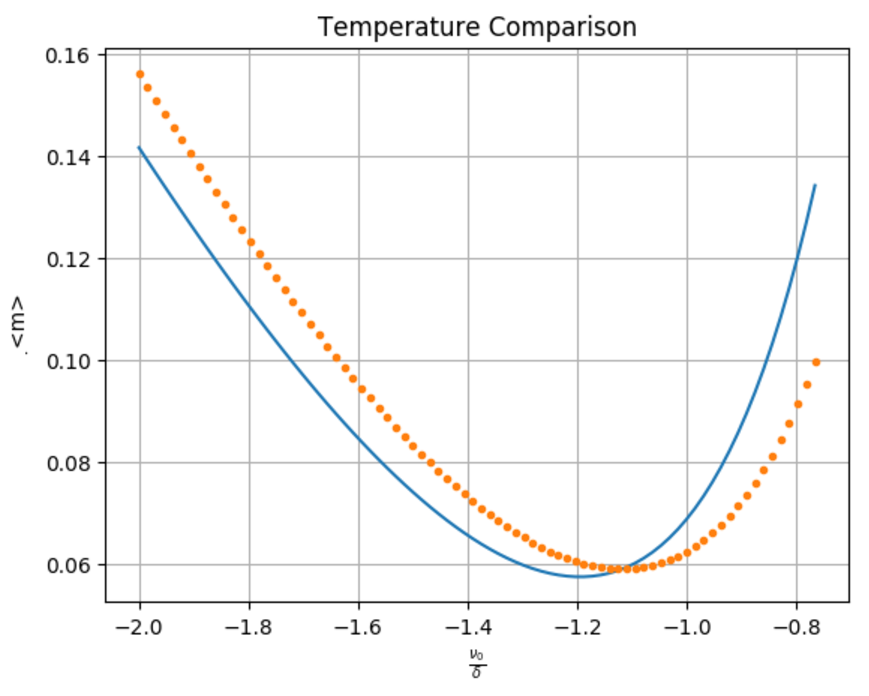
\includegraphics[scale=.80]{GraficaTemp.pdf} 
\caption{\textit{Comparación entre predicciones con y sin el término $\epsilon$} La línea puntuada representa la predicción sin dependencia temporal y la línea sólida representa la predicción con el término adicional.  Se utiliza $\kappa \ll \nu_0$}
\label{GraficaEnfriamiento}
\end{figure}

Como se observa en la figura \ref{GraficaEnfriamiento} claramente se obtiene un mínimo más pequeño de excitaciones posibles y un corrimiento en el punto donde se espera encontrar este mínimo. Esto correspondería a un mayor enfriamiento del espejo, pero no en los parámetros donde se esperaría encontrar sin la corrección.

\chapter{Enfriamiento Optomecánico Dependiente del Tiempo: Modelo Mejorado de Disipación Aplicado a Cavidad}

En el capítulo anterior se demostró, empleando un modelo mejorado de disipación, que si la frecuencia natural del oscilador armónico mecánico es una función periódica del tiempo, la temperatura final del oscilador es menor a la obtenida si no se utiliza el modelo mejorado. Este resultado motiva a investigar cual es la predicción respecto al estado final del sistema optomecánico cuando se emplea el modelo mejorado de disipación aplicado a la disipación de fotones a traves de los espejos de la cavidad cuando se considera que la frecuencia natural de esta es una función periódica del tiempo.
 
La frecuencia de natural de una cavidad de Fabry-Perot, asumiendo que su interior se encuentre en el vacío, está dada por

\begin{equation}
\nu_c = \frac{nc}{2L},
\end{equation} donde $c$ es la velocidad de la luz en el vacío, $n$ es algún entero positivo y $L$ es la longitud de la cavidad. Al emplear un montaje optomecánico como el que se lleva a los resultados del capítulo anterior, $L$ deja de ser constante. Si el oscilador mecánico tiene oscilaciones en torno a un punto de equilibrio dadas por $x_m(t)$ y se toma a $l_0$ como la longitud promedio de la cavidad, la longitud de la cavidad como función del tiempo está dada por

\begin{equation}
L(t) = l_0 + x_m(t)
\end{equation} lo cual lleva a una frecuencia 

\begin{align}
\nu_c(t) =& \frac{nc}{2l_0+2X_m(t)}, \\
\approx& \frac{nc}{2l_0} - \frac{nc X_m(t)}{4l_0^2}, \\
=& \frac{nc}{2l_0} - \frac{nc}{2l_0}(\frac{X_m(t)}{l_0}), \\
=& \omega_0 + \epsilon\omega_0C(t), \\
=& \omega_0(1+\epsilon\ C(t)).
\end{align} donde la expresión se deja en primer orden del parámetro de perturbación $\epsilon = \frac{x_m}{l_0}$ y la dependencia temporal de la amplitud queda contenida en $C(t)$, la cual también contiene un cambio de signo por simplicidad. Claramente la frecuencia natural de la cavidad es una función del tiempo. Esta dependencia usualmente no se toma en cuenta en los términos empleados para modelar la disipación de la cavidad. Para intentar resolver esto, intentamos modificar la disipación de la cavidad dada por el término ya antes visto

\begin{align}
L_a \rho =& - \frac{\kappa}{2}(n_p + 1)[a^\dagger a\rho + \rho a^\dagger a -2a\rho a^\dagger]  \\
 &- \frac{\kappa}{2}(n_p)[ aa^\dagger\rho + \rho  aa^\dagger -2a^\dagger\rho a].\nonumber
\end{align} 
el cual corresponde a una frecuencia natural constante.

Observamos que cuando se realiza la transformación unitaria
dada por los operadores de desplazamiento en la sección \ref{Desplazamiento}, el estado base en el nuevo marco de referencia corresponde al siguiente estado coherente

\begin{equation}
\Ket{\beta(t)}_D = e^{(\beta(t) b^\dagger - \beta(t)^*b)} \Ket{0},
\end{equation}  en el marco de referencia original. Esto quiere decir que al enfriar al oscilador armónico mecánico a una temperatura mínima el estado que se obtiene es muy cercano, en el marco desplazado, a
$\Ket{0}_D$, lo cual es muy cercano a un estado coherente en el marco
de referencia inicial. Suponemos entonces que el oscilador armónico
mecánico tiende, en la última etapa de enfriamiento, a un estado
del tipo


\begin{equation}
\Ket{\beta} + \epsilon\Ket{T}
\end{equation}


es decir a un estado coherente más una pequeña perturbación procedente
de ruido térmico. Proponemos emplear la frecuencia de este estado
coherente para  para modelar la disipación del campo dentro de la cavidad. Este proceso sería análogo a lo que se hizo con el oscilador optomecánico, pero aplicado a la pérdida de fotones desde dentro de la cavidad. Es importante notar que la frecuencia $\omega_\beta$ es constante durante este proceso, a diferencia de $\nu_c(t)$. Si el oscilador armónico mecánico se mueve de forma

\begin{equation}
x_m(t) = l_0 - xcos(\omega_\beta t)
\end{equation} se tiene que la frecuencia de la cavidad es

\begin{equation}
\nu_c(t) = \nu_0 + \epsilon cos(\omega_\beta t),
\end{equation} lo cual permite el uso de operadores de Floquet directamente en la disipación 

\begin{align}
L_\Gamma \rho =& - \frac{\kappa}{2}(n_c + 1)[\Gamma^\dagger \Gamma\rho + \rho \Gamma^\dagger \Gamma -2\Gamma\rho \Gamma^\dagger]  \\
 &- \frac{\kappa}{2}(n_c)[ \Gamma\Gamma^\dagger\rho + \rho  \Gamma\Gamma^\dagger -2\Gamma^\dagger\rho \Gamma].\nonumber
\end{align}

Este modelo de disipación es superior \cite{HanngiFM}, ya que toma en cuenta la variación periódica en la frecuencia natural del campo dentro de la cavidad, debido a que el oscilador mecánico continua su movimiento incluso cuando concluye el proceso de enfriamiento, por lo que la longitud de la cavidad nunca es constante.

Para trabajar con este modelo de disipación, sin embargo, es necesario modificar el Hamiltoniano. Los términos de disipación emergen de manera natural al deducir la ecuación maestra por lo que no sería correcto introducir este modelo de disipación de manera ad-hoc.  

Sin embargo, insertar estos operadores  de manera directa en el Hamiltoniano para la cavidad presenta varias complicaciones. Esto se debe a que los operadores de Floquet se expresan en términos de los operadores de posición y momento de un oscilador con frecuencia natural dependiente del tiempo, mientras que los operadores $a$ y $a^\dagger$ usuales corresponden a un oscilador sin esta dependencia. Si se asume que la frecuencia de la cavidad es su
frecuencia promedio y se expresan los operadores $a$ en términos de operadores de Floquet para sustituir en Hamiltoniano, se obtienen términos de la forma

\begin{equation}
a^\dagger a = C_1 (\nu_0, \omega_\beta)\Gamma^\dagger \Gamma + C_2(\nu_0, \omega_\beta) \Gamma \Gamma + C_3(\nu_0, \omega_\beta) \Gamma^\dagger \Gamma^\dagger +C_4(\nu_0, \omega_\beta) \Gamma \Gamma
\end{equation}

donde los coeficientes $C$ dependen de las dos frecuencias y de la
forma específica de las soluciones $f(t)$. El tratar de esta forma la
dependencia temporal de la cavidad presenta no solo complejidad añadida, también introduce una aproximación adicional. Esto señala la necesidad de intentar introducir los operadores de Floquet al Hamiltoniano desde primeros principios, después de lo cual
estos surgirán de manera natural en la disipación. Para entender mejor este procedimiento conviene entender la derivación del Hamiltoniano para una cavidad optomecánica. La derivación sigue el procedimiento de \cite{LawOH}.

\section{Ecuación de Onda para el Potencial Vectorial en una Cavidad con Espejo Móvil}

El potencial vectorial $A(x,t)$ dentro de la cavidad se define en la región $0 \leq x \leq q(t)$ donde $q(t)$ es la posición del espejo Esta coordenada es estrictamente no negativa y se toma el potencial $V(q)$ que siente el espejo como una barrera infinita en $q=0$. El potencial vectorial cumple la ecuación de onda con $c=1$

\begin{equation}\label{WaveEq}
\frac{\partial^2 A(x,t)}{\partial x^2} = \frac{\partial^2 A(x,t)}{\partial t^2},
\end{equation} con condiciones a la frontera que dependen del tiempo debido a la posición del espejo

\begin{equation}\label{VectorPotential}
A(0,t) = A(q(t),t) = 0.
\end{equation} Adicionalmente $q(t)$ cumple la ecuación

\begin{equation}\label{MirrorEq}
m\ddot{q} = -\frac{\partial V(q)}{\partial q} + \frac{1}{2}(\frac{\partial A(x,t)}{\partial x})^2 |_{x=q(t)}.
\end{equation} El segundo término del lado derecho es la presión de radiación que siente el espejo en su marco de referencia en reposo. La dinámica del sistema queda especificada por estas tres ecuaciones. Se define un juego de coordenadas generalizadas $Q_k$

\begin{equation} \label{QExpansion}
Q_k \equiv  \sqrt{\frac{2}{q(t)}} \int_0^{q(t)}dx A(x,t)sin(\frac{k\pi x}{q(t)}).
\end{equation} Esta expansión equivale a los distintos modos determinados por la posición instantánea del espejo. 

\begin{equation}
A(x,t) = \sum_{k=1}^\infty Q_k(t) \sqrt{\frac{2}{q(t)}}sin(\frac{k\pi x}{q(t)}).
\end{equation} Se puede sustituir esta expresión para $A(x,t)$ en \eqref{WaveEq},\eqref{MirrorEq}, \eqref{VectorPotential} y se obtiene dos ecuaciones

\begin{align}\label{RegularModesEq}
\ddot{Q}_k =& -\omega^2_k Q_k + 2\frac{\dot{q}}{q} \sum_j g_{kj}\dot{Q}_j +\frac{\ddot{q}q-\dot{q}^2}{q^2} \sum_j g_{kj}Q_j\\
&+ \frac{\dot{q}^2}{q^2}\sum_{j,l} g_{jk}g_{jl}Ql,\nonumber \\
m\ddot{q} =& -\frac{\partial V(q)}{\partial q} + \frac{1}{q}\sum_{k,j}(-1)^{k+j}\omega_k \omega_j Q_k Q_j.
\end{align} Las frecuencias $\omega_k$ están dadas por

\begin{equation}
\omega_k (q) = \frac{k\pi}{q},
\end{equation} y los coeficientes $g_{kj}$

\begin{align}
&(-1)^{k+j} \frac{2kj}{j^2-k^2}, k \neq j \\
g_{kj} = \Big \{\quad \nonumber &\\
& 0, k = j.\nonumber\\
\end{align} Estas ecuaciones son consecuencia de las ecuaciones de Euler-Lagrange del Lagrangiano 

\begin{align}
L(q,\dot{q},Q_k,\dot{Q}_k) =& \frac{1}{2} \sum_k [\dot{Q}_k^2-\omega_k^2(q)Q_k^2] + \frac{1}{2}m\dot{q}^2 - V(q)\\
&+\frac{\dot{q}}{q} \sum_{j,k} g_{kj}\dot{Q}_k Q_j + \frac{\dot{q}^2}{2q^2}\sum_{j,k,l} g_{kj}g_{kl}Q_l Q_j, \nonumber 
\end{align} de donde sigue el Hamiltoniano \eqref{LawHamiltonian} de manera directa. 

\begin{equation}\label{LawHamiltonian}
H = \frac{1}{2m}(p + \frac{g}{q} PQ)^2 + V(q) + \frac{1}{2}[P^2+\nu^2 (t)Q^2].
\end{equation} Los operadores $p$ y $q$ corresponden al oscilador mecánico y $P$ y $Q$ al campo dentro de la cavidad. $g$ es una constante. En el trabajo original la dependencia de la frecuencia es sobre la variable $q$ y no precisamente $t$. Se pide que la frecuencia $\nu(t)$ tenga una dependencia temporal periódica.

\section{Introduccion Directa de Operadores $\Gamma$ en el Hamiltoniano}

Se presenta un primer intento para introducir el formalismo de Floquet al Hamiltoniano de la cavidad y por ende a la disipación.  El teorema de Floquet permite obtener las soluciones de la ecuación

\begin{equation}\label{FloquetQ}
\ddot{Q} + \nu^2(t)Q=0,
\end{equation} y se les llama $f(t)$ y $f(t)^*$. De acuerdo con \cite{HanngiFM} los operadores de Floquet se pueden expresar como

\begin{equation}
\Gamma(t) = \frac{1}{2i}(Q\sqrt{\frac{2m}{\hbar}}\dot{f}(t)-P\sqrt{\frac{2}{m\hbar}}f(t))
\end{equation} y

\begin{equation}
\Gamma(t)^\dagger = \frac{-1}{2i}(Q\sqrt{\frac{2m}{\hbar}}\dot{f}^*(t)-P\sqrt{\frac{2}{m\hbar}}f^*(t)).
\end{equation} A futuro se omite la dependencia temporal de los operadores $\Gamma$ al darse por entendida. Se puede invertir el sistema de ecuaciones y obtener

\begin{align}
Q =& \frac{b^* \Gamma - b \Gamma^\dagger}{(b^* a - a^*b)},\\
P =& \frac{a^* \Gamma - a \Gamma^\dagger}{(b^* a - a^*b)}.
\end{align} donde

\begin{align}
a =& \frac{1}{2i}\sqrt{\frac{2m}{\hbar}} \dot{f}(t),\\
b =& \frac{1}{2i}\sqrt{\frac{2}{m\hbar}} f(t).
\end{align} Esto se sustituye en el término $PQ$ del Hamiltoniano y se obtiene

\begin{equation}
H = \frac{1}{2m}(p + g \gamma)^2 + v(q) + \frac{1}{2}[P^2+\nu^2 (t)Q^2],
\end{equation} donde

\begin{equation}
\gamma = \frac{\hbar^2}{W^2 q}[ab^*\Gamma^\dagger \Gamma + a^*b \Gamma \Gamma^\dagger - a^*b^* \Gamma \Gamma - ab \Gamma^\dagger \Gamma^\dagger]
\end{equation} con

\begin{equation}
W= \frac{\dot{f}(t)f^*(t)-\dot{f}^*(t)f(t)}{2i}.
\end{equation}
Esto contrasta con la aproximación realizada en el trabajo original \cite{LawOH}
donde los operadores de creación y aniquilación de la cavidad se
expanden en una serie de potencias para aproximar la dependencia de
estos sobre el operador $q$ del oscilador mecánico. En este
procedimiento se asume $q = l_o + x_m$.  Se hace la aproximación de tomar al término $\gamma$ en el punto promedio  $q=l_0$


Para simplificar con el primer término del Hamiltoniano se emplea la transformación unitaria dada por el operador

\begin{equation}
T = e^\frac{i x_m \gamma}{\hbar}.
\end{equation} Bajo esta transformación 

\begin{align*}
T^\dagger p T =& p - \gamma, \\
T^\dagger p^2 T =& p^2 -2p\gamma, \\
T^\dagger \gamma T =& \gamma,
\end{align*} por lo que, despreciando el término $\gamma^2$ por ser del orden de $\frac{1}{l_0^2}$

\begin{equation}
\frac{1}{2m}(p + g \gamma)^2 \approx \frac{p^2}{2m}.
\end{equation} Se conoce que, expresados en operadores de Floquet, los operadores $P$ y $Q$ corresponden a un Hamiltoniano con la forma funcional de un oscilador armónico cuántico usual. Por esto, queda aplicar la transformación al término $\Gamma^\dagger \Gamma$. Cortando a primer orden en $\epsilon$

\begin{align*}
e^{\frac{-ix\gamma_0}{\hbar}}\Gamma^\dagger \Gamma e^{\frac{ix_m\gamma_0}{\hbar}} =& \Gamma^\dagger \Gamma + \frac{ix_m}{\hbar}[\Gamma^\dagger \Gamma, \gamma_0], \\
=& \Gamma^\dagger \Gamma + \frac{2i\hbar x_m}{W^2 l_0}(a^*b \Gamma^\dagger \Gamma + a^*b^* \Gamma \Gamma -ab\Gamma^\dagger \Gamma^\dagger),\\
\approx & \Gamma^\dagger \Gamma + \frac{2i\hbar x_m}{W^2 l_0} a^*b \Gamma^\dagger \Gamma, \\
=& \Gamma^\dagger \Gamma - \frac{i \dot{f}^*(t)f(t) }{W^2 l_0} x_m  \Gamma^\dagger \Gamma,
\end{align*} de esta forma la constante de proporcionalidad de la presión de radiación es una cantidad dependiente del tiempo bajo este enfoque. Esto contrasta con la definición usual $F= \frac{\omega_0 \hbar}{l_0}$. Solo se trabaja con los operadores de número al estar en una aproximación de un solo modo. Tomando en cuenta el factor de amplitud global para el Hamiltoniano de oscilador armónico con frecuencia natural dependiente del tiempo $\frac{W}{|f(t)|^2}$ se obtiene

\begin{equation}
H_{cav} = \frac{\hbar W}{|f(t)|^2}\Gamma^\dagger \Gamma - \frac{\hbar i\dot{f}^*(t)f(t) }{|f(t)|^2W l_0}x  \Gamma^ \dagger \Gamma,
\end{equation} lo cual lleva a identificar el nuevo coeficiente de fuerza $F$ el cual es ahora una función del tiempo

\begin{equation}
F(t) = \frac{\hbar i\dot{f}^*(t)f(t) }{|f(t)|^2W l_0},
\end{equation} y a un Hamiltoniano para un oscilador optomecánico de la forma

\begin{equation}
H = \hbar \omega b^\dagger b + \hbar\frac{ W}{|f(t)|^2}\Gamma^\dagger \Gamma -F(t)x_m\Gamma^\dagger \Gamma,
\end{equation} pero $x_m$ es el operador de posición del espejo, el cual se puede expresar en términos de los operadores de creación y aniquilación del oscilador armónico mecánico

\begin{equation}
H = \hbar \omega b^\dagger b + \hbar\frac{ W}{|f(t)|^2}\Gamma^\dagger \Gamma -g(t)\Gamma^\dagger \Gamma(b^\dagger + b),
\end{equation} donde $g$ es una función del tiempo que modula la fuerza de la interacción y está dada por

\begin{equation}
g(t) = \sqrt{\frac{\hbar}{2m\omega}}F(t).
\end{equation} 
A este Hamiltoniano se le agrega un término correspondiente a un láser de forzamiento

\begin{equation}
H_{laser}= \hbar \frac{\Omega}{2}(\Gamma^\dagger + \Gamma).
\end{equation} Y lleva a un Hamiltoniano completo

\begin{equation}
H = \hbar \omega b^\dagger b + \hbar\frac{ W}{|f(t)|^2}\Gamma^\dagger \Gamma -g(t)\Gamma^\dagger \Gamma(b^\dagger + b) + \hbar \frac{\Omega}{2}(\Gamma^\dagger + \Gamma).
\end{equation} Este Hamiltoniano asume que el cambio en la longitud de la cavidad es lo suficientemente lento para que el campo dentro de la misma se mantenga en un solo modo y asume que este modo corresponde a un movimiento periódico del oscilador mecánico. El siguiente paso en el proyecto es encontrar la solución para el comportamiento de $x_m(t)$ para así poder determinar la frecuencia natural de la cavidad y la forma explícita de los operadores de Floquet.


 La ecuación maestra que corresponde a este Hamiltoniano toma en cuenta los intercambios de energía del sistema con el ambiente, tanto la pérdida de fotones de la cavidad como la re-termalización del oscilador mecánico. Esta es \cite{BarberisLC}

\begin{equation} \label{LCMasterEquation}
\dot{\rho} = \frac{1}{i\hbar}[H,\rho] +L_b\rho + L_\Gamma \rho
\end{equation}

Los términos $L$ representan los intercambios de energía con el ambiente. Corresponden al oscilador mecánico y a la cavidad respectivamente. De forma explícita

\begin{align}
L_b \rho =& - \frac{\gamma}{2}(n_m + 1)[b^\dagger b\rho + \rho b^\dagger b -2b\rho b^\dagger]  \\
 &- \frac{\gamma}{2}(n_m)[ bb^\dagger\rho + \rho  bb^\dagger -2b^\dagger\rho b].\nonumber
\end{align} 

\begin{align}
L_\Gamma \rho =& - \frac{\kappa}{2}(n_c + 1)[\Gamma^\dagger \Gamma\rho + \rho \Gamma^\dagger \Gamma -2\Gamma\rho \Gamma^\dagger]  \\
 &- \frac{\kappa}{2}(n_c)[ \Gamma\Gamma^\dagger\rho + \rho  \Gamma\Gamma^\dagger -2\Gamma^\dagger\rho \Gamma].\nonumber
\end{align}

$n_m$ y $n_c$ representan el número promedio de excitaciones térmicas y $\gamma$ y $\kappa$ modelan la pérdida de energía ante el ambiente. 

Esta derivación lleva a un resultado interesante, sin embargo existen problemas de compatibilidad con las ecuaciones originales en \cite{LawOH}. El problema consiste en que aplicar el formalismo de Floquet impone dos condiciones. 

\begin{enumerate}
\item Impone que el oscilador armónico mecánico realice un movimiento armónico simple. Esta es una condición que equivale a conocer la solución para el movimiento descrito por $q$ durante la derivación de las ecuaciones.

\item La solución para $Q$ debe cumplir con dos ecuaciones, \eqref{RegularModesEq} y \eqref{FloquetQ}. Sería necesario encontrar una solución única que cumpliera con ambas ecuaciones. 
\end{enumerate}

Esto señala la necesidad de introducir el formalismo de Floquet en una etapa anterior de la derivación del Hamiltoniano. El candidato más evidente es la ecuación \eqref{QExpansion}. Buscaremos una expansión distinta a la utilizada en este caso, a fin de generar ecuaciones compatibles con el formalismo de Floquet. Una vez el Hamiltoniano queda expresado con estos operadores, se puede utilizar el modelo de disipación correspondiente en el caso de la cavidad.



\section{Transformación al Marco de Referencia Desplazado}

Esta transformación se utiliza para eliminar términos de orden tercero en operadores en la ecuación \eqref{LCMasterEquation}. La transformación es unitaria y se genera mediante el operador

\begin{equation}
U_{b,\Gamma} =  U_b U_\Gamma = e^{(\beta b^\dagger - \beta^* b)}e^{(\alpha\Gamma^\dagger - \alpha^* \Gamma)}.
\end{equation} $\alpha$ y $\beta$ son coeficientes complejos dependientes del tiempo que se elijen de manera conveniente para simplificar la ecuación maestra. Se busca una ecuación para la matriz densidad no transformada \cite{TesisMaestria}. Bajo la transformación la matriz densidad es

\begin{equation}
\rho' = U_{b,\Gamma}^\dagger \rho U_{b,\Gamma}.
\end{equation} Se puede despejar en términos de $\rho$, utilizando el hecho de que la transformación es unitaria

\begin{equation}
\rho = U_{b,\Gamma} \rho' U_{b,\Gamma}^\dagger,
\end{equation}y derivando respecto al tiempo

\begin{equation}
\dot{\rho} = L\rho = \frac{d}{dt}(U_{b,\Gamma} \rho' U_{b,\Gamma}^\dagger).
\end{equation} En este caso, $L$ representa el operador de Liouville. Esto permite obtener una ecuación maestra para $\rho'$. 

\begin{align}
 U_{b,\Gamma} \dot{(\rho')} U_{b,\Gamma}^\dagger =& L[U_{b,\Gamma} \rho' U_{b,\Gamma}^\dagger] - \dot{U}_{b,\Gamma}\rho'U_{b,\Gamma}^\dagger -U_{b,\Gamma} \rho' \dot{U}_{b,\Gamma}^\dagger\\
\dot{\rho} =& U_{b,\Gamma}^\dagger L[U_{b,\Gamma} \rho' U_{b,\Gamma}^\dagger]U_{b,\Gamma}-U_{b,\Gamma}^\dagger\dot{U}_{b,\Gamma}\rho'-\rho'\dot{U}_{b,\Gamma}^\dagger U_{b,\Gamma}.
\end{align} A partir de este punto, se omiten los sub-índices de las transformaciones y la $'$ para la matriz densidad. La transformación afecta a los distintos operadores presentes en el Hamiltoniano de la siguiente forma

\begin{align}
U^\dagger b U =& b + \beta,\\
U^\dagger \Gamma U =& \Gamma + \alpha,\\
U^\dagger b^\dagger b U =& b^\dagger b + \alpha^* b + \alpha b^\dagger +|\beta|^2,\\
U^\dagger \Gamma^\dagger \Gamma U =& \Gamma^\dagger \Gamma + \alpha^* \Gamma + \alpha \Gamma^\dagger +|\alpha|^2.
\end{align} Los conjugados Hermitianos se obtienen de manera trivial. Utilizar operadores con dependencia temporal explícita añade complejidad adicional a este procedimiento debido a las derivadas temporales del operador $U$. El procedimiento completo puede encontrarse en \cite{TesisMaestria}. Se obtiene

\begin{align}
\dot{U}_b=&\dot{\beta} b^\dagger U_b - U_b\dot{\beta}^*b - \frac{1}{2}(\dot{\beta} \beta^*+\dot{\beta}^* \beta)U_b,\\
\dot{U}_b^\dagger=&-\dot{\beta} b^\dagger U_b^\dagger + U_b^\dagger\dot{\beta}^*b - \frac{1}{2}(\dot{\beta} \beta^*+\dot{\beta}^* \beta)U_b^\dagger.
\end{align} El caso de $U_\Gamma$ es más complejo, pero el procedimiento es equivalente. Se obtiene

\begin{align}
\dot{U}_\Gamma =&(\dot{\alpha}\Gamma^\dagger +\alpha \dot{\Gamma}^\dagger)U_\Gamma - U_\Gamma(\dot{\alpha}^*\Gamma+\alpha^* \dot{\Gamma}) + (\alpha^*)^2 C_{--}(t)U_\Gamma-\frac{1}{2}(\dot{\alpha} \alpha^*+\dot{\alpha}^* \alpha)U_\Gamma, \\
\dot{U}^\dagger_\Gamma=&-(\dot{\alpha}\Gamma^\dagger +\alpha \dot{\Gamma}^\dagger)U_\Gamma^\dagger + U_\Gamma^\dagger(\dot{\alpha}^*\Gamma+\alpha^* \dot{\Gamma}) - (\alpha)^2 C_{++}(t)U_\Gamma^\dagger-\frac{1}{2}(\dot{\alpha} \alpha^*+\dot{\alpha}^* \alpha)U_\Gamma^\dagger.
\end{align} Finalmente se debe calcular las transformaciones de las derivadas temporales de los operadores $\Gamma$

\begin{align}
U^{\dagger}\dot{\Gamma}U =& \dot{\Gamma} + \alpha C_{-+}(t) -\alpha^* C_{--}(t),\\
U^{\dagger}\dot{\Gamma}^\dagger U =& \dot{\Gamma}^\dagger - \alpha^* C_{+-}(t) +\alpha C_{++}(t). 
\end{align} Los coeficientes $C(t)$ surgen debido a que los operadores $\Gamma$ no necesariamente conmutan con sus derivadas temporales

\begin{align*}
C_{++}(t) =& [\dot{\Gamma}^{\dagger}, \Gamma^{\dagger}],\\
C_{+-}(t) =& [\dot{\Gamma}^{\dagger}, \Gamma],\\
C_{-+}(t) =& [\dot{\Gamma}, \Gamma^{\dagger}],\\
C_{--}(t) =& [\dot{\Gamma}, \Gamma].
\end{align*} Falta únicamente calcular los términos de la ecuación maestra que corresponden a estas derivadas temporales

\begin{equation}
U_b^\dagger \dot{U}_b \rho + U_\Gamma^\dagger \dot{U}_\Gamma \rho + \rho \dot{U}_b^\dagger U_b+ \rho \dot{U}_\Gamma^\dagger U_\Gamma,
\end{equation} los cuales resultan ser

\begin{align}
U_\Gamma^\dagger \dot{U}_\Gamma \rho &= [(\dot{\alpha}\Gamma^\dagger + \alpha \dot{\Gamma}^\dagger - \dot{\alpha}^*\Gamma -\alpha^*\dot{\Gamma} ) \\
 &- |\alpha|^2C_{+-} + (\alpha)^2C_{++} + (\alpha^*)^2 C_{--} - \frac{1}{2}\dot{|\alpha^2|} + \dot{\alpha}^*\alpha]\rho \nonumber,
\end{align}

\begin{align}
 \rho \dot{U}_\Gamma^\dagger U_\Gamma &= \rho[(-\dot{\alpha}\Gamma^\dagger - \alpha \dot{\Gamma}^\dagger + \dot{\alpha}^*\Gamma +\alpha^*\dot{\Gamma} ) \\
 &+ |\alpha|^2C_{-+} - (\alpha)^2C_{++} - (\alpha^*)^2 C_{--} - \frac{1}{2}\dot{|\alpha^2|} + \dot{\alpha}\alpha^*], \nonumber
\end{align}

\begin{align}
U_\Gamma^\dagger \dot{U}_\Gamma \rho + \rho \dot{U}_\Gamma^\dagger U_\Gamma &= [\rho, (\alpha^*\dot{\Gamma} - \alpha\dot{\Gamma}^\dagger)] + [\rho, (\dot{\alpha}^*\Gamma - \dot{\alpha}\Gamma^\dagger)] \\
&+|\alpha|^2 (C_{-+} - C_{+-}).
\end{align} 

Los términos que involucran un conmutador con la matriz densidad se consideran parte del Hamiltoniano. El procedimiento para los términos  $U_b$ es el mismo pero resulta más sencillo

\begin{equation}
U_b^\dagger \dot{U}_b \rho+ \rho \dot{U}_b^\dagger U_b = [\rho, (\dot{\beta}^*b - \dot{\beta}b^\dagger)].
\end{equation} El Hamiltoniano queda entonces dado por

\begin{align}
H_{mec}' =& \hbar \omega(b^{\dagger}b +\beta b^{\dagger}+\beta^* b + |\beta|^2),\\
H_{cav}' =& \hbar\frac{W}{|f(t)|^2}(\Gamma^{\dagger}\Gamma + \alpha \Gamma^{\dagger} + \alpha^* \Gamma + |\alpha|^2 ),\\
H_{rad}'=&-\hbar g(t)[(\Gamma^{\dagger}\Gamma + \alpha \Gamma^{\dagger} + \alpha^* \Gamma + |\alpha|^2 )((b^{\dagger}+\beta^*)+(b+\beta))],\\
B' =& \frac{\hbar \Omega}{2}(\Gamma^{\dagger} + \Gamma +\alpha + \alpha^*).
\end{align}

Más términos adicionales generados por la transformación debido a sus derivadas temporales

\begin{equation}
H_{T} = (\alpha^*\dot{\Gamma} - \alpha\dot{\Gamma}^\dagger) +(\dot{\alpha}^*\Gamma - \dot{\alpha}\Gamma^\dagger) +(\dot{\beta}^*b - \dot{\beta}b^\dagger),
\end{equation} y debido a los términos de Lindblad

\begin{equation}
U^\dagger [L_aU\rho U^\dagger]U + U^\dagger [L_\Gamma U\rho U^\dagger]U,
\end{equation} se generan términos adicionales para el Hamiltoniano mientras que los términos de Lindblad mantienen su forma original

\begin{align}
U^\dagger [L_bU\rho U^\dagger]U=& L_b\rho + [\beta b^\dagger - \beta^* b,\rho],\\
U^\dagger [L_\Gamma U\rho U^\dagger]U =& L_\Gamma \rho + [ \alpha \Gamma^\dagger - \alpha^* \Gamma,\rho].
\end{align} La transformación de los términos Lindblad resulta en  Hamiltoniano efectivo adicional

\begin{equation}
H_L = -\frac{\gamma}{2}(\beta b^\dagger + \beta^* b) -\frac{\kappa}{2}( \alpha \Gamma^\dagger + \alpha^* \Gamma).
\end{equation} A fin de simplificar el Hamiltoniano, es necesario agrupar todos los términos a primer orden en operadores

\begin{align}
&b(\omega\beta - g(t)|\alpha|^2 + i\dot{\beta}^* + i\frac{\gamma}{2}\beta),\\
&\Gamma(\frac{W\alpha}{|f|^2} -g(t)\alpha(\beta^*+\beta) + \frac{\Omega}{2}-i\dot{\alpha} - i\frac{\kappa}{2}\alpha),
\end{align} y sus conjugados Hermitianos. Para anular estos términos es necesario que se cumpla el sistema de ecuaciones diferenciales

\begin{align}
&\dot{\beta} = -i\omega\beta^* + ig(t)|\alpha|^2 - \frac{\gamma}{2}\beta,\\
&\dot{\alpha} = -i \frac{W}{|f|^2}\alpha^* + ig(t)\alpha(\beta + \beta^*) -i \frac{\Omega}{2} - \frac{\kappa}{2}\alpha^*.
\end{align} Debido a la forma de la frecuencia elegida, la función $f(t)$ que figura en los operadores $\Gamma$ es

\begin{equation}
f(t) = e^{i\omega t} + \frac{\epsilon}{16}e^{3i\omega t}
\end{equation} por lo que si se desprecian términos de corrección menores a epsilon

\begin{align}
\dot{\Gamma}(t) =& i\omega \Gamma(t),\\
\dot{\Gamma}^\dagger(t) =& -i\omega \Gamma^\dagger(t),
\end{align} y estos términos deben incluirse en las ecuaciones para $\alpha$ y $\beta$

\begin{align}
&\dot{\beta} = -i\omega\beta^* + ig(t)|\alpha|^2 - \frac{\gamma}{2}\beta,\\
&\dot{\alpha} = -i \frac{W}{|f|^2}\alpha^* + ig(t)\alpha(\beta + \beta^*) -i \frac{\Omega}{2} - \frac{\kappa}{2}\alpha^* + \omega\alpha^*.
\end{align} El caso de interés es el caso estacionario $\dot{\alpha}=\dot{\beta} = 0$. Se trabaja el límite de acoplamiento pequeño y se limita el análisis a orden 0 en el parámetro de acoplamiento $g(t)$

\begin{align}
&0 = -i\omega\beta^* - \frac{\gamma}{2}\beta,\\
&0 = -i \frac{W}{|f|^2}\alpha^* -i \frac{\Omega}{2} - \frac{\kappa}{2}\alpha^* + \omega\alpha^*.
\end{align} dada la expresión para $f(t)$ se tiene

\begin{equation}
\frac{W}{|f(t)|^2} = \omega,
\end{equation} se llega a la solución, a orden 0 en acoplamiento

\begin{align}
\beta_0 =& 0, \\
\alpha_0 =& \frac{\Omega}{-i\kappa - 2\omega(1-i)}.
\end{align} lo cual resulta en el Hamiltoniano transformado

\begin{equation}
H = \hbar \omega b^\dagger b + \hbar\omega \Gamma^\dagger \Gamma -\hbar g(t)[( \alpha \Gamma^{\dagger} + \alpha^* \Gamma)(b^{\dagger}+b)]
\end{equation} donde se ha despreciado el término $\Gamma^{\dagger}\Gamma$ en la interacción ya que en este régimen $|\alpha| \gg 1$ y es despreciable respecto a los otros dos términos. De esta forma se tiene un nuevo Hamiltoniano para interacción optomecánica donde se modela que la intensidad de la interacción optomecánica es una función del tiempo.

\chapter{Objetivos Futuros}


A partir del Hamiltoniano \eqref{LCHamiltonian} es posible estudiar un sistema de gran importancia tomando en cuenta su dependencia temporal inherente, la cual se no se toma en cuenta en los modelos de disipación usuales\cite{CavesIF}. A partir de este punto se proponen tres objetivos para realizar un estudio más completo de este sistema bajo este nuevo enfoque. En todos los casos se espera obtener expresiones analíticas y resultados numéricos  para la temperatura final del oscilador mecánico bajo la aproximación adiabática.

\section{Objetivos y Calendarización}

\begin{enumerate}
\item Llegar a una expresión para la temperatura final del espejo bajo la aproximación adiabática y compararla con la expresión usual que se obtiene al no considerar una dependencia temporal explícita para la frecuencia natural de la cavidad en la disipación. Esto requiere deducir desde primeros principios la ecuación maestra que contiene los coeficientes de enfriamiento y calentamiento correspondientes al oscilador mecánico así como resolver el movimiento del oscilador armónico mecánico.

\item Estudiar el sistema en un régimen distinto al establecido en los capítulos anteriores. Si no se puede tomar la interacción a orden cero durante la transformación al marco desplazado esto cambia el coeficiente $\alpha$ y lo convierte en una función del tiempo.

\item Estudiar el sistema cuando el parámetro $\epsilon$ debe tomarse en cuenta hasta segundo orden. Este cambio lleva a que incluso el factor global del Hamiltoniano para el campo dentro de la cavidad sea una función del tiempo, lo que lleva a estudiar el efecto sobre el oscilador de interactuar con un campo cuya frecuencia natural oscila en el tiempo. 
\end{enumerate}

Se asume que cada uno de estos objetivos, junto con trabajo de redacción y revisión bibliográfica adicional, sea realizable dentro de un semestre de trabajo. Esto implicaría un último semestre únicamente dedicado a redacción a fin de elaborar la tesis doctoral en tiempo y forma, así como un artículo de investigación a ser publicado en una revista internacional.

\bibliographystyle{unsrt}
\bibliography{Bib}

\end{document}
